\documentclass[11pt]{article}

% Camera-ready (final) mode: no review option, no line numbers (organizer's instruction).
\usepackage{acl}
\usepackage{times}
\usepackage{latexsym}
\usepackage[T1]{fontenc}
\usepackage[utf8]{inputenc}
\usepackage{microtype}
\usepackage{graphicx}
\usepackage{booktabs}
\usepackage{amsmath}
\usepackage{multirow}
\usepackage{xcolor}
\usepackage{enumitem}
\makeatletter\g@addto@macro\UrlBreaks{\do\-}\makeatother  % long Hub paths wrap at hyphens
\setlist{nosep,leftmargin=*}

% Every number in the text is a \V{key} looked up in numbers.tex (written by make_assets.py from result files).
% An undefined key prints a red ??key and a LaTeX warning, so a missing number can never pass silently.
\makeatletter
\newcommand{\V}[1]{\ifcsname v@#1\endcsname\csname v@#1\endcsname\else
  \textcolor{red}{\textbf{??\detokenize{#1}}}\@latex@warning{Undefined value #1}\fi}
\makeatother
% Generated by paper/make_assets.py. Do not edit by hand.
\expandafter\def\csname v@cfg.a1.n\endcsname{1000}
\expandafter\def\csname v@cfg.a2.benign\endcsname{900}
\expandafter\def\csname v@cfg.a2.harmful\endcsname{100}
\expandafter\def\csname v@cfg.a3.klmax\endcsname{0.1}
\expandafter\def\csname v@cfg.a3.nharm\endcsname{32}
\expandafter\def\csname v@cfg.am.epochs\endcsname{2}
\expandafter\def\csname v@cfg.am.k\endcsname{6}
\expandafter\def\csname v@cfg.am.layers\endcsname{2, 3, 4, 5, 6, 7}
\expandafter\def\csname v@cfg.am.lr\endcsname{1\times10^{-4}}
\expandafter\def\csname v@cfg.am.shieldbits\endcsname{8}
\expandafter\def\csname v@cfg.batch_size\endcsname{4}
\expandafter\def\csname v@cfg.bon.n\endcsname{8}
\expandafter\def\csname v@cfg.bon.sigma\endcsname{0.4}
\expandafter\def\csname v@cfg.cap.arc_challenge\endcsname{500}
\expandafter\def\csname v@cfg.cap.gsm8k\endcsname{250}
\expandafter\def\csname v@cfg.cap.hellaswag\endcsname{500}
\expandafter\def\csname v@cfg.cap.winogrande\endcsname{500}
\expandafter\def\csname v@cfg.effbatch\endcsname{16}
\expandafter\def\csname v@cfg.epochs\endcsname{1}
\expandafter\def\csname v@cfg.grad_accum\endcsname{4}
\expandafter\def\csname v@cfg.hqq.group\endcsname{64}
\expandafter\def\csname v@cfg.lora_alpha\endcsname{32}
\expandafter\def\csname v@cfg.lora_r\endcsname{16}
\expandafter\def\csname v@cfg.lr\endcsname{2\times10^{-4}}
\expandafter\def\csname v@cfg.max_len\endcsname{512}
\expandafter\def\csname v@cfg.mj.n\endcsname{100}
\expandafter\def\csname v@cfg.ml.harmful\endcsname{100}
\expandafter\def\csname v@cfg.ml.xstest\endcsname{50}
\expandafter\def\csname v@cfg.n.calib\endcsname{64}
\expandafter\def\csname v@cfg.n.harmful\endcsname{200}
\expandafter\def\csname v@cfg.n.mmlu\endcsname{300}
\expandafter\def\csname v@cfg.n.xstest\endcsname{250}
\expandafter\def\csname v@cfg.sr.n\endcsname{150}
\expandafter\def\csname v@hum.humanrate.kw.afive\endcsname{31}
\expandafter\def\csname v@hum.humanrate.kw.all\endcsname{40}
\expandafter\def\csname v@hum.humanrate.kw.other\endcsname{51}
\expandafter\def\csname v@hum.humanrate.kwref.all\endcsname{43}
\expandafter\def\csname v@hum.humanrate.lg.afive\endcsname{14}
\expandafter\def\csname v@hum.humanrate.lg.all\endcsname{21}
\expandafter\def\csname v@hum.humanrate.lg.other\endcsname{29}
\expandafter\def\csname v@hum.humanrate.wg.afive\endcsname{14}
\expandafter\def\csname v@hum.humanrate.wg.all\endcsname{21}
\expandafter\def\csname v@hum.humanrate.wg.other\endcsname{29}
\expandafter\def\csname v@hum.humanrate.wgref.all\endcsname{43}
\expandafter\def\csname v@hum.n.kw.afive\endcsname{42}
\expandafter\def\csname v@hum.n.kw.all\endcsname{77}
\expandafter\def\csname v@hum.n.kw.other\endcsname{35}
\expandafter\def\csname v@hum.n.kwref.all\endcsname{23}
\expandafter\def\csname v@hum.n.lg.afive\endcsname{42}
\expandafter\def\csname v@hum.n.lg.all\endcsname{77}
\expandafter\def\csname v@hum.n.lg.other\endcsname{35}
\expandafter\def\csname v@hum.n.wg.afive\endcsname{42}
\expandafter\def\csname v@hum.n.wg.all\endcsname{77}
\expandafter\def\csname v@hum.n.wg.other\endcsname{35}
\expandafter\def\csname v@hum.n.wgref.all\endcsname{23}
\expandafter\def\csname v@hum.nlabels\endcsname{103}
\expandafter\def\csname v@hum.rate.kw.afive\endcsname{93}
\expandafter\def\csname v@hum.rate.kw.all\endcsname{87}
\expandafter\def\csname v@hum.rate.kw.other\endcsname{80}
\expandafter\def\csname v@hum.rate.kwref.all\endcsname{13}
\expandafter\def\csname v@hum.rate.lg.afive\endcsname{71}
\expandafter\def\csname v@hum.rate.lg.all\endcsname{62}
\expandafter\def\csname v@hum.rate.lg.other\endcsname{51}
\expandafter\def\csname v@hum.rate.wg.afive\endcsname{29}
\expandafter\def\csname v@hum.rate.wg.all\endcsname{38}
\expandafter\def\csname v@hum.rate.wg.other\endcsname{49}
\expandafter\def\csname v@hum.rate.wgref.all\endcsname{48}
\expandafter\def\csname v@kappa.kw.afive\endcsname{0.07}
\expandafter\def\csname v@kappa.kw.all\endcsname{0.18}
\expandafter\def\csname v@kappa.kw.other\endcsname{0.42}
\expandafter\def\csname v@kappa.kwref.all\endcsname{0.33}
\expandafter\def\csname v@kappa.lg.afive\endcsname{0.05}
\expandafter\def\csname v@kappa.lg.all\endcsname{0.09}
\expandafter\def\csname v@kappa.lg.other\endcsname{0.21}
\expandafter\def\csname v@kappa.wg.afive\endcsname{0.18}
\expandafter\def\csname v@kappa.wg.all\endcsname{0.42}
\expandafter\def\csname v@kappa.wg.other\endcsname{0.60}
\expandafter\def\csname v@kappa.wgref.all\endcsname{0.91}
\expandafter\def\csname v@lg.A0.fixes.max\endcsname{14}
\expandafter\def\csname v@lg.A0.fixes.min\endcsname{1}
\expandafter\def\csname v@lg.A2.max\endcsname{86}
\expandafter\def\csname v@lg.A2.min\endcsname{80}
\expandafter\def\csname v@lg.AM.A0\endcsname{1}
\expandafter\def\csname v@lg.AM.A0.ci\endcsname{[0, 2]}
\expandafter\def\csname v@lg.AM.A1\endcsname{8}
\expandafter\def\csname v@lg.AM.A1.ci\endcsname{[4, 12]}
\expandafter\def\csname v@lg.AM.A2\endcsname{86}
\expandafter\def\csname v@lg.AM.A2.ci\endcsname{[81, 90]}
\expandafter\def\csname v@lg.AM.A3\endcsname{79}
\expandafter\def\csname v@lg.AM.A3.ci\endcsname{[73, 84]}
\expandafter\def\csname v@lg.AM.A3max\endcsname{79}
\expandafter\def\csname v@lg.AM.A3max.ci\endcsname{[73, 84]}
\expandafter\def\csname v@lg.AM.A4q3\endcsname{4}
\expandafter\def\csname v@lg.AM.A4q3.ci\endcsname{[2, 8]}
\expandafter\def\csname v@lg.AM.A5bon\endcsname{68}
\expandafter\def\csname v@lg.AM.A5bon.ci\endcsname{[62, 74]}
\expandafter\def\csname v@lg.AM.A5raw\endcsname{57}
\expandafter\def\csname v@lg.AM.A5raw.ci\endcsname{[50, 64]}
\expandafter\def\csname v@lg.AM_all.A0\endcsname{0}
\expandafter\def\csname v@lg.AM_all.A0.ci\endcsname{[0, 2]}
\expandafter\def\csname v@lg.AM_all.A2\endcsname{88}
\expandafter\def\csname v@lg.AM_all.A2.ci\endcsname{[84, 92]}
\expandafter\def\csname v@lg.AM_all.A3\endcsname{0}
\expandafter\def\csname v@lg.AM_all.A3.ci\endcsname{[0, 2]}
\expandafter\def\csname v@lg.AM_all.A3max\endcsname{62}
\expandafter\def\csname v@lg.AM_all.A3max.ci\endcsname{[56, 69]}
\expandafter\def\csname v@lg.AM_rand0.A0\endcsname{0}
\expandafter\def\csname v@lg.AM_rand0.A0.ci\endcsname{[0, 2]}
\expandafter\def\csname v@lg.AM_rand0.A2\endcsname{88}
\expandafter\def\csname v@lg.AM_rand0.A2.ci\endcsname{[83, 92]}
\expandafter\def\csname v@lg.AM_rand0.A3\endcsname{76}
\expandafter\def\csname v@lg.AM_rand0.A3.ci\endcsname{[70, 82]}
\expandafter\def\csname v@lg.AM_rand0.A3max\endcsname{76}
\expandafter\def\csname v@lg.AM_rand0.A3max.ci\endcsname{[70, 82]}
\expandafter\def\csname v@lg.AM_rand1.A0\endcsname{0}
\expandafter\def\csname v@lg.AM_rand1.A0.ci\endcsname{[0, 2]}
\expandafter\def\csname v@lg.AM_rand1.A2\endcsname{88}
\expandafter\def\csname v@lg.AM_rand1.A2.ci\endcsname{[83, 92]}
\expandafter\def\csname v@lg.AM_rand1.A3\endcsname{1}
\expandafter\def\csname v@lg.AM_rand1.A3.ci\endcsname{[0, 2]}
\expandafter\def\csname v@lg.AM_rand1.A3max\endcsname{54}
\expandafter\def\csname v@lg.AM_rand1.A3max.ci\endcsname{[46, 60]}
\expandafter\def\csname v@lg.BASE.A0\endcsname{8}
\expandafter\def\csname v@lg.BASE.A0.ci\endcsname{[5, 12]}
\expandafter\def\csname v@lg.BASE.A1\endcsname{8}
\expandafter\def\csname v@lg.BASE.A1.ci\endcsname{[4, 12]}
\expandafter\def\csname v@lg.BASE.A2\endcsname{81}
\expandafter\def\csname v@lg.BASE.A2.ci\endcsname{[76, 86]}
\expandafter\def\csname v@lg.BASE.A3\endcsname{70}
\expandafter\def\csname v@lg.BASE.A3.ci\endcsname{[63, 76]}
\expandafter\def\csname v@lg.BASE.A3max\endcsname{70}
\expandafter\def\csname v@lg.BASE.A3max.ci\endcsname{[63, 76]}
\expandafter\def\csname v@lg.BASE.A4q3\endcsname{14}
\expandafter\def\csname v@lg.BASE.A4q3.ci\endcsname{[9, 18]}
\expandafter\def\csname v@lg.BASE.A4q4\endcsname{10}
\expandafter\def\csname v@lg.BASE.A4q4.ci\endcsname{[6, 14]}
\expandafter\def\csname v@lg.BASE.A5bon\endcsname{95}
\expandafter\def\csname v@lg.BASE.A5bon.ci\endcsname{[92, 98]}
\expandafter\def\csname v@lg.BASE.A5raw\endcsname{56}
\expandafter\def\csname v@lg.BASE.A5raw.ci\endcsname{[50, 63]}
\expandafter\def\csname v@lg.GC.A0\endcsname{1}
\expandafter\def\csname v@lg.GC.A0.ci\endcsname{[0, 2]}
\expandafter\def\csname v@lg.GC.A1\endcsname{6}
\expandafter\def\csname v@lg.GC.A1.ci\endcsname{[4, 10]}
\expandafter\def\csname v@lg.GC.A2\endcsname{82}
\expandafter\def\csname v@lg.GC.A2.ci\endcsname{[77, 88]}
\expandafter\def\csname v@lg.GC.A3\endcsname{10}
\expandafter\def\csname v@lg.GC.A3.ci\endcsname{[6, 14]}
\expandafter\def\csname v@lg.GC.A3max\endcsname{10}
\expandafter\def\csname v@lg.GC.A3max.ci\endcsname{[6, 14]}
\expandafter\def\csname v@lg.GC.A4q3\endcsname{1}
\expandafter\def\csname v@lg.GC.A4q3.ci\endcsname{[0, 2]}
\expandafter\def\csname v@lg.GC.A4q4\endcsname{0}
\expandafter\def\csname v@lg.GC.A4q4.ci\endcsname{[0, 2]}
\expandafter\def\csname v@lg.GC.A5bon\endcsname{29}
\expandafter\def\csname v@lg.GC.A5bon.ci\endcsname{[22, 36]}
\expandafter\def\csname v@lg.GC.A5raw\endcsname{45}
\expandafter\def\csname v@lg.GC.A5raw.ci\endcsname{[38, 52]}
\expandafter\def\csname v@lg.IL.A0\endcsname{8}
\expandafter\def\csname v@lg.IL.A0.ci\endcsname{[4, 12]}
\expandafter\def\csname v@lg.IL.A1\endcsname{10}
\expandafter\def\csname v@lg.IL.A1.ci\endcsname{[6, 15]}
\expandafter\def\csname v@lg.IL.A2\endcsname{86}
\expandafter\def\csname v@lg.IL.A2.ci\endcsname{[82, 91]}
\expandafter\def\csname v@lg.IL.A3\endcsname{68}
\expandafter\def\csname v@lg.IL.A3.ci\endcsname{[61, 74]}
\expandafter\def\csname v@lg.IL.A3max\endcsname{68}
\expandafter\def\csname v@lg.IL.A3max.ci\endcsname{[61, 74]}
\expandafter\def\csname v@lg.IL.A4q3\endcsname{11}
\expandafter\def\csname v@lg.IL.A4q3.ci\endcsname{[7, 16]}
\expandafter\def\csname v@lg.IL.A4q4\endcsname{8}
\expandafter\def\csname v@lg.IL.A4q4.ci\endcsname{[4, 12]}
\expandafter\def\csname v@lg.IL.A5bon\endcsname{94}
\expandafter\def\csname v@lg.IL.A5bon.ci\endcsname{[90, 97]}
\expandafter\def\csname v@lg.IL.A5raw\endcsname{52}
\expandafter\def\csname v@lg.IL.A5raw.ci\endcsname{[45, 58]}
\expandafter\def\csname v@lg.RL.A0\endcsname{3}
\expandafter\def\csname v@lg.RL.A0.ci\endcsname{[1, 6]}
\expandafter\def\csname v@lg.RL.A1\endcsname{2}
\expandafter\def\csname v@lg.RL.A1.ci\endcsname{[0, 4]}
\expandafter\def\csname v@lg.RL.A2\endcsname{81}
\expandafter\def\csname v@lg.RL.A2.ci\endcsname{[76, 86]}
\expandafter\def\csname v@lg.RL.A3\endcsname{6}
\expandafter\def\csname v@lg.RL.A3.ci\endcsname{[3, 10]}
\expandafter\def\csname v@lg.RL.A3max\endcsname{33}
\expandafter\def\csname v@lg.RL.A3max.ci\endcsname{[26, 40]}
\expandafter\def\csname v@lg.RL.A4q3\endcsname{4}
\expandafter\def\csname v@lg.RL.A4q3.ci\endcsname{[2, 8]}
\expandafter\def\csname v@lg.RL.A5bon\endcsname{55}
\expandafter\def\csname v@lg.RL.A5bon.ci\endcsname{[48, 62]}
\expandafter\def\csname v@lg.RL.A5raw\endcsname{56}
\expandafter\def\csname v@lg.RL.A5raw.ci\endcsname{[50, 63]}
\expandafter\def\csname v@lg.RL_noguard.A0\endcsname{8}
\expandafter\def\csname v@lg.RL_noguard.A0.ci\endcsname{[5, 12]}
\expandafter\def\csname v@lg.RL_noguard.A1\endcsname{8}
\expandafter\def\csname v@lg.RL_noguard.A1.ci\endcsname{[4, 12]}
\expandafter\def\csname v@lg.RL_noguard.A2\endcsname{81}
\expandafter\def\csname v@lg.RL_noguard.A2.ci\endcsname{[76, 86]}
\expandafter\def\csname v@lg.RL_noguard.A3\endcsname{70}
\expandafter\def\csname v@lg.RL_noguard.A3.ci\endcsname{[63, 76]}
\expandafter\def\csname v@lg.RL_noguard.A3max\endcsname{70}
\expandafter\def\csname v@lg.RL_noguard.A3max.ci\endcsname{[63, 76]}
\expandafter\def\csname v@lg.RL_noguard.A4q3\endcsname{14}
\expandafter\def\csname v@lg.RL_noguard.A4q3.ci\endcsname{[9, 18]}
\expandafter\def\csname v@lg.RL_noguard.A5bon\endcsname{95}
\expandafter\def\csname v@lg.RL_noguard.A5bon.ci\endcsname{[92, 98]}
\expandafter\def\csname v@lg.RL_noguard.A5raw\endcsname{56}
\expandafter\def\csname v@lg.RL_noguard.A5raw.ci\endcsname{[50, 63]}
\expandafter\def\csname v@lg.SDT.A0\endcsname{14}
\expandafter\def\csname v@lg.SDT.A0.ci\endcsname{[10, 20]}
\expandafter\def\csname v@lg.SDT.A1\endcsname{21}
\expandafter\def\csname v@lg.SDT.A1.ci\endcsname{[16, 26]}
\expandafter\def\csname v@lg.SDT.A2\endcsname{85}
\expandafter\def\csname v@lg.SDT.A2.ci\endcsname{[80, 90]}
\expandafter\def\csname v@lg.SDT.A3\endcsname{16}
\expandafter\def\csname v@lg.SDT.A3.ci\endcsname{[10, 20]}
\expandafter\def\csname v@lg.SDT.A3max\endcsname{83}
\expandafter\def\csname v@lg.SDT.A3max.ci\endcsname{[78, 88]}
\expandafter\def\csname v@lg.SDT.A4q3\endcsname{15}
\expandafter\def\csname v@lg.SDT.A4q3.ci\endcsname{[10, 20]}
\expandafter\def\csname v@lg.SDT.A5bon\endcsname{96}
\expandafter\def\csname v@lg.SDT.A5bon.ci\endcsname{[94, 99]}
\expandafter\def\csname v@lg.SDT.A5raw\endcsname{74}
\expandafter\def\csname v@lg.SDT.A5raw.ci\endcsname{[68, 80]}
\expandafter\def\csname v@lg.SP.A0\endcsname{6}
\expandafter\def\csname v@lg.SP.A0.ci\endcsname{[3, 10]}
\expandafter\def\csname v@lg.SP.A1\endcsname{10}
\expandafter\def\csname v@lg.SP.A1.ci\endcsname{[6, 14]}
\expandafter\def\csname v@lg.SP.A2\endcsname{80}
\expandafter\def\csname v@lg.SP.A2.ci\endcsname{[74, 86]}
\expandafter\def\csname v@lg.SP.A3\endcsname{82}
\expandafter\def\csname v@lg.SP.A3.ci\endcsname{[77, 88]}
\expandafter\def\csname v@lg.SP.A3max\endcsname{82}
\expandafter\def\csname v@lg.SP.A3max.ci\endcsname{[77, 88]}
\expandafter\def\csname v@lg.SP.A4q3\endcsname{10}
\expandafter\def\csname v@lg.SP.A4q3.ci\endcsname{[6, 15]}
\expandafter\def\csname v@lg.SP.A5bon\endcsname{96}
\expandafter\def\csname v@lg.SP.A5bon.ci\endcsname{[94, 99]}
\expandafter\def\csname v@lg.SP.A5raw\endcsname{60}
\expandafter\def\csname v@lg.SP.A5raw.ci\endcsname{[54, 66]}
\expandafter\def\csname v@lg.ST.A0\endcsname{10}
\expandafter\def\csname v@lg.ST.A0.ci\endcsname{[6, 14]}
\expandafter\def\csname v@lg.ST.A1\endcsname{28}
\expandafter\def\csname v@lg.ST.A1.ci\endcsname{[22, 34]}
\expandafter\def\csname v@lg.ST.A2\endcsname{81}
\expandafter\def\csname v@lg.ST.A2.ci\endcsname{[76, 86]}
\expandafter\def\csname v@lg.ST.A3\endcsname{42}
\expandafter\def\csname v@lg.ST.A3.ci\endcsname{[34, 48]}
\expandafter\def\csname v@lg.ST.A3max\endcsname{42}
\expandafter\def\csname v@lg.ST.A3max.ci\endcsname{[35, 48]}
\expandafter\def\csname v@lg.ST.A4q3\endcsname{8}
\expandafter\def\csname v@lg.ST.A4q3.ci\endcsname{[4, 12]}
\expandafter\def\csname v@lg.ST.A5bon\endcsname{96}
\expandafter\def\csname v@lg.ST.A5bon.ci\endcsname{[92, 98]}
\expandafter\def\csname v@lg.ST.A5raw\endcsname{73}
\expandafter\def\csname v@lg.ST.A5raw.ci\endcsname{[67, 79]}
\expandafter\def\csname v@mmlu.AM.A0\endcsname{52}
\expandafter\def\csname v@mmlu.AM.A0.ci\endcsname{[47, 58]}
\expandafter\def\csname v@mmlu.AM.A1\endcsname{53}
\expandafter\def\csname v@mmlu.AM.A1.ci\endcsname{[48, 59]}
\expandafter\def\csname v@mmlu.AM.A2\endcsname{54}
\expandafter\def\csname v@mmlu.AM.A2.ci\endcsname{[48, 60]}
\expandafter\def\csname v@mmlu.AM.A3\endcsname{52}
\expandafter\def\csname v@mmlu.AM.A3.ci\endcsname{[46, 58]}
\expandafter\def\csname v@mmlu.AM.A3max\endcsname{52}
\expandafter\def\csname v@mmlu.AM.A3max.ci\endcsname{[46, 58]}
\expandafter\def\csname v@mmlu.AM.A4q3\endcsname{50}
\expandafter\def\csname v@mmlu.AM.A4q3.ci\endcsname{[44, 56]}
\expandafter\def\csname v@mmlu.AM.A5raw\endcsname{39}
\expandafter\def\csname v@mmlu.AM.A5raw.ci\endcsname{[33, 45]}
\expandafter\def\csname v@mmlu.AM_all.A0\endcsname{54}
\expandafter\def\csname v@mmlu.AM_all.A0.ci\endcsname{[48, 59]}
\expandafter\def\csname v@mmlu.AM_all.A2\endcsname{54}
\expandafter\def\csname v@mmlu.AM_all.A2.ci\endcsname{[48, 60]}
\expandafter\def\csname v@mmlu.AM_all.A3\endcsname{54}
\expandafter\def\csname v@mmlu.AM_all.A3.ci\endcsname{[49, 60]}
\expandafter\def\csname v@mmlu.AM_all.A3max\endcsname{52}
\expandafter\def\csname v@mmlu.AM_all.A3max.ci\endcsname{[47, 58]}
\expandafter\def\csname v@mmlu.AM_rand0.A0\endcsname{53}
\expandafter\def\csname v@mmlu.AM_rand0.A0.ci\endcsname{[47, 58]}
\expandafter\def\csname v@mmlu.AM_rand0.A2\endcsname{55}
\expandafter\def\csname v@mmlu.AM_rand0.A2.ci\endcsname{[50, 61]}
\expandafter\def\csname v@mmlu.AM_rand0.A3\endcsname{54}
\expandafter\def\csname v@mmlu.AM_rand0.A3.ci\endcsname{[48, 59]}
\expandafter\def\csname v@mmlu.AM_rand0.A3max\endcsname{54}
\expandafter\def\csname v@mmlu.AM_rand0.A3max.ci\endcsname{[48, 59]}
\expandafter\def\csname v@mmlu.AM_rand1.A0\endcsname{54}
\expandafter\def\csname v@mmlu.AM_rand1.A0.ci\endcsname{[48, 59]}
\expandafter\def\csname v@mmlu.AM_rand1.A2\endcsname{55}
\expandafter\def\csname v@mmlu.AM_rand1.A2.ci\endcsname{[49, 60]}
\expandafter\def\csname v@mmlu.AM_rand1.A3\endcsname{55}
\expandafter\def\csname v@mmlu.AM_rand1.A3.ci\endcsname{[49, 61]}
\expandafter\def\csname v@mmlu.AM_rand1.A3max\endcsname{52}
\expandafter\def\csname v@mmlu.AM_rand1.A3max.ci\endcsname{[47, 58]}
\expandafter\def\csname v@mmlu.BASE.A0\endcsname{53}
\expandafter\def\csname v@mmlu.BASE.A0.ci\endcsname{[47, 58]}
\expandafter\def\csname v@mmlu.BASE.A1\endcsname{56}
\expandafter\def\csname v@mmlu.BASE.A1.ci\endcsname{[50, 61]}
\expandafter\def\csname v@mmlu.BASE.A2\endcsname{55}
\expandafter\def\csname v@mmlu.BASE.A2.ci\endcsname{[49, 61]}
\expandafter\def\csname v@mmlu.BASE.A3\endcsname{53}
\expandafter\def\csname v@mmlu.BASE.A3.ci\endcsname{[47, 58]}
\expandafter\def\csname v@mmlu.BASE.A3max\endcsname{53}
\expandafter\def\csname v@mmlu.BASE.A3max.ci\endcsname{[47, 58]}
\expandafter\def\csname v@mmlu.BASE.A4q3\endcsname{49}
\expandafter\def\csname v@mmlu.BASE.A4q3.ci\endcsname{[43, 54]}
\expandafter\def\csname v@mmlu.BASE.A4q4\endcsname{52}
\expandafter\def\csname v@mmlu.BASE.A4q4.ci\endcsname{[46, 58]}
\expandafter\def\csname v@mmlu.BASE.A5raw\endcsname{44}
\expandafter\def\csname v@mmlu.BASE.A5raw.ci\endcsname{[38, 50]}
\expandafter\def\csname v@mmlu.GC.A0\endcsname{54}
\expandafter\def\csname v@mmlu.GC.A0.ci\endcsname{[49, 60]}
\expandafter\def\csname v@mmlu.GC.A1\endcsname{52}
\expandafter\def\csname v@mmlu.GC.A1.ci\endcsname{[46, 57]}
\expandafter\def\csname v@mmlu.GC.A2\endcsname{53}
\expandafter\def\csname v@mmlu.GC.A2.ci\endcsname{[48, 59]}
\expandafter\def\csname v@mmlu.GC.A3\endcsname{52}
\expandafter\def\csname v@mmlu.GC.A3.ci\endcsname{[47, 58]}
\expandafter\def\csname v@mmlu.GC.A3max\endcsname{52}
\expandafter\def\csname v@mmlu.GC.A3max.ci\endcsname{[47, 58]}
\expandafter\def\csname v@mmlu.GC.A4q3\endcsname{46}
\expandafter\def\csname v@mmlu.GC.A4q3.ci\endcsname{[41, 52]}
\expandafter\def\csname v@mmlu.GC.A4q4\endcsname{54}
\expandafter\def\csname v@mmlu.GC.A4q4.ci\endcsname{[48, 60]}
\expandafter\def\csname v@mmlu.GC.A5raw\endcsname{30}
\expandafter\def\csname v@mmlu.GC.A5raw.ci\endcsname{[24, 35]}
\expandafter\def\csname v@mmlu.IL.A0\endcsname{54}
\expandafter\def\csname v@mmlu.IL.A0.ci\endcsname{[48, 59]}
\expandafter\def\csname v@mmlu.IL.A1\endcsname{54}
\expandafter\def\csname v@mmlu.IL.A1.ci\endcsname{[48, 59]}
\expandafter\def\csname v@mmlu.IL.A2\endcsname{55}
\expandafter\def\csname v@mmlu.IL.A2.ci\endcsname{[49, 60]}
\expandafter\def\csname v@mmlu.IL.A3\endcsname{53}
\expandafter\def\csname v@mmlu.IL.A3.ci\endcsname{[48, 59]}
\expandafter\def\csname v@mmlu.IL.A3max\endcsname{53}
\expandafter\def\csname v@mmlu.IL.A3max.ci\endcsname{[48, 59]}
\expandafter\def\csname v@mmlu.IL.A4q3\endcsname{49}
\expandafter\def\csname v@mmlu.IL.A4q3.ci\endcsname{[43, 55]}
\expandafter\def\csname v@mmlu.IL.A4q4\endcsname{52}
\expandafter\def\csname v@mmlu.IL.A4q4.ci\endcsname{[46, 57]}
\expandafter\def\csname v@mmlu.IL.A5raw\endcsname{31}
\expandafter\def\csname v@mmlu.IL.A5raw.ci\endcsname{[26, 36]}
\expandafter\def\csname v@mmlu.RL.A0\endcsname{53}
\expandafter\def\csname v@mmlu.RL.A0.ci\endcsname{[47, 59]}
\expandafter\def\csname v@mmlu.RL.A1\endcsname{54}
\expandafter\def\csname v@mmlu.RL.A1.ci\endcsname{[49, 60]}
\expandafter\def\csname v@mmlu.RL.A2\endcsname{54}
\expandafter\def\csname v@mmlu.RL.A2.ci\endcsname{[49, 60]}
\expandafter\def\csname v@mmlu.RL.A3\endcsname{56}
\expandafter\def\csname v@mmlu.RL.A3.ci\endcsname{[51, 62]}
\expandafter\def\csname v@mmlu.RL.A3max\endcsname{53}
\expandafter\def\csname v@mmlu.RL.A3max.ci\endcsname{[47, 58]}
\expandafter\def\csname v@mmlu.RL.A4q3\endcsname{48}
\expandafter\def\csname v@mmlu.RL.A4q3.ci\endcsname{[42, 54]}
\expandafter\def\csname v@mmlu.RL.A5raw\endcsname{44}
\expandafter\def\csname v@mmlu.RL.A5raw.ci\endcsname{[38, 50]}
\expandafter\def\csname v@mmlu.RL_noguard.A0\endcsname{53}
\expandafter\def\csname v@mmlu.RL_noguard.A0.ci\endcsname{[47, 58]}
\expandafter\def\csname v@mmlu.RL_noguard.A1\endcsname{56}
\expandafter\def\csname v@mmlu.RL_noguard.A1.ci\endcsname{[50, 61]}
\expandafter\def\csname v@mmlu.RL_noguard.A2\endcsname{55}
\expandafter\def\csname v@mmlu.RL_noguard.A2.ci\endcsname{[49, 61]}
\expandafter\def\csname v@mmlu.RL_noguard.A3\endcsname{53}
\expandafter\def\csname v@mmlu.RL_noguard.A3.ci\endcsname{[47, 58]}
\expandafter\def\csname v@mmlu.RL_noguard.A3max\endcsname{53}
\expandafter\def\csname v@mmlu.RL_noguard.A3max.ci\endcsname{[47, 58]}
\expandafter\def\csname v@mmlu.RL_noguard.A4q3\endcsname{49}
\expandafter\def\csname v@mmlu.RL_noguard.A4q3.ci\endcsname{[43, 54]}
\expandafter\def\csname v@mmlu.RL_noguard.A5raw\endcsname{44}
\expandafter\def\csname v@mmlu.RL_noguard.A5raw.ci\endcsname{[38, 50]}
\expandafter\def\csname v@mmlu.SDT.A0\endcsname{54}
\expandafter\def\csname v@mmlu.SDT.A0.ci\endcsname{[48, 60]}
\expandafter\def\csname v@mmlu.SDT.A1\endcsname{54}
\expandafter\def\csname v@mmlu.SDT.A1.ci\endcsname{[48, 60]}
\expandafter\def\csname v@mmlu.SDT.A2\endcsname{53}
\expandafter\def\csname v@mmlu.SDT.A2.ci\endcsname{[47, 59]}
\expandafter\def\csname v@mmlu.SDT.A3\endcsname{55}
\expandafter\def\csname v@mmlu.SDT.A3.ci\endcsname{[49, 60]}
\expandafter\def\csname v@mmlu.SDT.A3max\endcsname{54}
\expandafter\def\csname v@mmlu.SDT.A3max.ci\endcsname{[48, 60]}
\expandafter\def\csname v@mmlu.SDT.A4q3\endcsname{48}
\expandafter\def\csname v@mmlu.SDT.A4q3.ci\endcsname{[43, 54]}
\expandafter\def\csname v@mmlu.SDT.A5raw\endcsname{38}
\expandafter\def\csname v@mmlu.SDT.A5raw.ci\endcsname{[33, 44]}
\expandafter\def\csname v@mmlu.SP.A0\endcsname{53}
\expandafter\def\csname v@mmlu.SP.A0.ci\endcsname{[47, 59]}
\expandafter\def\csname v@mmlu.SP.A1\endcsname{55}
\expandafter\def\csname v@mmlu.SP.A1.ci\endcsname{[49, 60]}
\expandafter\def\csname v@mmlu.SP.A2\endcsname{54}
\expandafter\def\csname v@mmlu.SP.A2.ci\endcsname{[49, 60]}
\expandafter\def\csname v@mmlu.SP.A3\endcsname{55}
\expandafter\def\csname v@mmlu.SP.A3.ci\endcsname{[49, 60]}
\expandafter\def\csname v@mmlu.SP.A3max\endcsname{55}
\expandafter\def\csname v@mmlu.SP.A3max.ci\endcsname{[49, 60]}
\expandafter\def\csname v@mmlu.SP.A4q3\endcsname{50}
\expandafter\def\csname v@mmlu.SP.A4q3.ci\endcsname{[44, 56]}
\expandafter\def\csname v@mmlu.SP.A5raw\endcsname{42}
\expandafter\def\csname v@mmlu.SP.A5raw.ci\endcsname{[36, 48]}
\expandafter\def\csname v@mmlu.ST.A0\endcsname{47}
\expandafter\def\csname v@mmlu.ST.A0.ci\endcsname{[41, 53]}
\expandafter\def\csname v@mmlu.ST.A1\endcsname{53}
\expandafter\def\csname v@mmlu.ST.A1.ci\endcsname{[48, 59]}
\expandafter\def\csname v@mmlu.ST.A2\endcsname{51}
\expandafter\def\csname v@mmlu.ST.A2.ci\endcsname{[46, 57]}
\expandafter\def\csname v@mmlu.ST.A3\endcsname{44}
\expandafter\def\csname v@mmlu.ST.A3.ci\endcsname{[39, 50]}
\expandafter\def\csname v@mmlu.ST.A3max\endcsname{44}
\expandafter\def\csname v@mmlu.ST.A3max.ci\endcsname{[39, 50]}
\expandafter\def\csname v@mmlu.ST.A4q3\endcsname{40}
\expandafter\def\csname v@mmlu.ST.A4q3.ci\endcsname{[34, 45]}
\expandafter\def\csname v@mmlu.ST.A5raw\endcsname{22}
\expandafter\def\csname v@mmlu.ST.A5raw.ci\endcsname{[18, 27]}
\expandafter\def\csname v@or.AM.A0\endcsname{7}
\expandafter\def\csname v@or.AM.A0.ci\endcsname{[4, 10]}
\expandafter\def\csname v@or.AM.A1\endcsname{6}
\expandafter\def\csname v@or.AM.A1.ci\endcsname{[4, 10]}
\expandafter\def\csname v@or.AM.A2\endcsname{1}
\expandafter\def\csname v@or.AM.A2.ci\endcsname{[0, 2]}
\expandafter\def\csname v@or.AM.A3\endcsname{0}
\expandafter\def\csname v@or.AM.A3.ci\endcsname{[0, 1]}
\expandafter\def\csname v@or.AM.A4q3\endcsname{11}
\expandafter\def\csname v@or.AM.A4q3.ci\endcsname{[7, 15]}
\expandafter\def\csname v@or.AM_all.A0\endcsname{11}
\expandafter\def\csname v@or.AM_all.A0.ci\endcsname{[7, 15]}
\expandafter\def\csname v@or.AM_all.A2\endcsname{1}
\expandafter\def\csname v@or.AM_all.A2.ci\endcsname{[0, 2]}
\expandafter\def\csname v@or.AM_all.A3\endcsname{12}
\expandafter\def\csname v@or.AM_all.A3.ci\endcsname{[8, 16]}
\expandafter\def\csname v@or.AM_rand0.A0\endcsname{11}
\expandafter\def\csname v@or.AM_rand0.A0.ci\endcsname{[7, 15]}
\expandafter\def\csname v@or.AM_rand0.A2\endcsname{1}
\expandafter\def\csname v@or.AM_rand0.A2.ci\endcsname{[0, 3]}
\expandafter\def\csname v@or.AM_rand0.A3\endcsname{1}
\expandafter\def\csname v@or.AM_rand0.A3.ci\endcsname{[0, 2]}
\expandafter\def\csname v@or.AM_rand1.A0\endcsname{9}
\expandafter\def\csname v@or.AM_rand1.A0.ci\endcsname{[6, 12]}
\expandafter\def\csname v@or.AM_rand1.A2\endcsname{1}
\expandafter\def\csname v@or.AM_rand1.A2.ci\endcsname{[0, 2]}
\expandafter\def\csname v@or.AM_rand1.A3\endcsname{10}
\expandafter\def\csname v@or.AM_rand1.A3.ci\endcsname{[7, 14]}
\expandafter\def\csname v@or.BASE.A0\endcsname{9}
\expandafter\def\csname v@or.BASE.A0.ci\endcsname{[6, 13]}
\expandafter\def\csname v@or.BASE.A1\endcsname{4}
\expandafter\def\csname v@or.BASE.A1.ci\endcsname{[2, 7]}
\expandafter\def\csname v@or.BASE.A2\endcsname{2}
\expandafter\def\csname v@or.BASE.A2.ci\endcsname{[0, 4]}
\expandafter\def\csname v@or.BASE.A3\endcsname{2}
\expandafter\def\csname v@or.BASE.A3.ci\endcsname{[0, 4]}
\expandafter\def\csname v@or.BASE.A4q3\endcsname{6}
\expandafter\def\csname v@or.BASE.A4q3.ci\endcsname{[4, 10]}
\expandafter\def\csname v@or.BASE.A5raw\endcsname{4}
\expandafter\def\csname v@or.BASE.A5raw.ci\endcsname{[2, 7]}
\expandafter\def\csname v@or.GC.A0\endcsname{26}
\expandafter\def\csname v@or.GC.A0.ci\endcsname{[21, 32]}
\expandafter\def\csname v@or.GC.A1\endcsname{6}
\expandafter\def\csname v@or.GC.A1.ci\endcsname{[3, 9]}
\expandafter\def\csname v@or.GC.A2\endcsname{1}
\expandafter\def\csname v@or.GC.A2.ci\endcsname{[0, 3]}
\expandafter\def\csname v@or.GC.A3\endcsname{17}
\expandafter\def\csname v@or.GC.A3.ci\endcsname{[12, 22]}
\expandafter\def\csname v@or.GC.A4q3\endcsname{27}
\expandafter\def\csname v@or.GC.A4q3.ci\endcsname{[22, 32]}
\expandafter\def\csname v@or.GC.A5raw\endcsname{18}
\expandafter\def\csname v@or.GC.A5raw.ci\endcsname{[13, 22]}
\expandafter\def\csname v@or.IL.A0\endcsname{10}
\expandafter\def\csname v@or.IL.A0.ci\endcsname{[6, 14]}
\expandafter\def\csname v@or.IL.A1\endcsname{5}
\expandafter\def\csname v@or.IL.A1.ci\endcsname{[3, 8]}
\expandafter\def\csname v@or.IL.A2\endcsname{2}
\expandafter\def\csname v@or.IL.A2.ci\endcsname{[0, 3]}
\expandafter\def\csname v@or.IL.A3\endcsname{0}
\expandafter\def\csname v@or.IL.A3.ci\endcsname{[0, 1]}
\expandafter\def\csname v@or.IL.A4q3\endcsname{12}
\expandafter\def\csname v@or.IL.A4q3.ci\endcsname{[8, 16]}
\expandafter\def\csname v@or.IL.A5raw\endcsname{4}
\expandafter\def\csname v@or.IL.A5raw.ci\endcsname{[2, 7]}
\expandafter\def\csname v@or.RL.A0\endcsname{18}
\expandafter\def\csname v@or.RL.A0.ci\endcsname{[14, 23]}
\expandafter\def\csname v@or.RL.A1\endcsname{17}
\expandafter\def\csname v@or.RL.A1.ci\endcsname{[12, 22]}
\expandafter\def\csname v@or.RL.A2\endcsname{8}
\expandafter\def\csname v@or.RL.A2.ci\endcsname{[5, 12]}
\expandafter\def\csname v@or.RL.A3\endcsname{19}
\expandafter\def\csname v@or.RL.A3.ci\endcsname{[14, 24]}
\expandafter\def\csname v@or.RL.A4q3\endcsname{26}
\expandafter\def\csname v@or.RL.A4q3.ci\endcsname{[21, 32]}
\expandafter\def\csname v@or.RL.A5raw\endcsname{4}
\expandafter\def\csname v@or.RL.A5raw.ci\endcsname{[2, 7]}
\expandafter\def\csname v@or.RL_noguard.A0\endcsname{9}
\expandafter\def\csname v@or.RL_noguard.A0.ci\endcsname{[6, 13]}
\expandafter\def\csname v@or.RL_noguard.A1\endcsname{4}
\expandafter\def\csname v@or.RL_noguard.A1.ci\endcsname{[2, 7]}
\expandafter\def\csname v@or.RL_noguard.A2\endcsname{2}
\expandafter\def\csname v@or.RL_noguard.A2.ci\endcsname{[0, 4]}
\expandafter\def\csname v@or.RL_noguard.A3\endcsname{2}
\expandafter\def\csname v@or.RL_noguard.A3.ci\endcsname{[0, 4]}
\expandafter\def\csname v@or.RL_noguard.A4q3\endcsname{6}
\expandafter\def\csname v@or.RL_noguard.A4q3.ci\endcsname{[4, 10]}
\expandafter\def\csname v@or.RL_noguard.A5raw\endcsname{4}
\expandafter\def\csname v@or.RL_noguard.A5raw.ci\endcsname{[2, 7]}
\expandafter\def\csname v@or.SDT.A0\endcsname{2}
\expandafter\def\csname v@or.SDT.A0.ci\endcsname{[1, 4]}
\expandafter\def\csname v@or.SDT.A1\endcsname{2}
\expandafter\def\csname v@or.SDT.A1.ci\endcsname{[0, 3]}
\expandafter\def\csname v@or.SDT.A2\endcsname{1}
\expandafter\def\csname v@or.SDT.A2.ci\endcsname{[0, 2]}
\expandafter\def\csname v@or.SDT.A3\endcsname{4}
\expandafter\def\csname v@or.SDT.A3.ci\endcsname{[2, 6]}
\expandafter\def\csname v@or.SDT.A4q3\endcsname{3}
\expandafter\def\csname v@or.SDT.A4q3.ci\endcsname{[1, 6]}
\expandafter\def\csname v@or.SDT.A5raw\endcsname{4}
\expandafter\def\csname v@or.SDT.A5raw.ci\endcsname{[2, 6]}
\expandafter\def\csname v@or.SP.A0\endcsname{10}
\expandafter\def\csname v@or.SP.A0.ci\endcsname{[6, 14]}
\expandafter\def\csname v@or.SP.A1\endcsname{5}
\expandafter\def\csname v@or.SP.A1.ci\endcsname{[2, 8]}
\expandafter\def\csname v@or.SP.A2\endcsname{2}
\expandafter\def\csname v@or.SP.A2.ci\endcsname{[0, 3]}
\expandafter\def\csname v@or.SP.A3\endcsname{1}
\expandafter\def\csname v@or.SP.A3.ci\endcsname{[0, 3]}
\expandafter\def\csname v@or.SP.A4q3\endcsname{7}
\expandafter\def\csname v@or.SP.A4q3.ci\endcsname{[4, 11]}
\expandafter\def\csname v@or.SP.A5raw\endcsname{4}
\expandafter\def\csname v@or.SP.A5raw.ci\endcsname{[2, 7]}
\expandafter\def\csname v@or.ST.A0\endcsname{21}
\expandafter\def\csname v@or.ST.A0.ci\endcsname{[16, 26]}
\expandafter\def\csname v@or.ST.A1\endcsname{4}
\expandafter\def\csname v@or.ST.A1.ci\endcsname{[2, 6]}
\expandafter\def\csname v@or.ST.A2\endcsname{2}
\expandafter\def\csname v@or.ST.A2.ci\endcsname{[0, 4]}
\expandafter\def\csname v@or.ST.A3\endcsname{4}
\expandafter\def\csname v@or.ST.A3.ci\endcsname{[2, 6]}
\expandafter\def\csname v@or.ST.A4q3\endcsname{39}
\expandafter\def\csname v@or.ST.A4q3.ci\endcsname{[33, 45]}
\expandafter\def\csname v@or.ST.A5raw\endcsname{14}
\expandafter\def\csname v@or.ST.A5raw.ci\endcsname{[10, 18]}
\expandafter\def\csname v@ov.e6harmful100.exact\endcsname{0}
\expandafter\def\csname v@ov.e6harmful100.flagged\endcsname{1}
\expandafter\def\csname v@ov.e6harmful100.maxcos\endcsname{0.92}
\expandafter\def\csname v@ov.e6harmful100.maxjac\endcsname{0.33}
\expandafter\def\csname v@ov.harmfultest.exact\endcsname{0}
\expandafter\def\csname v@ov.harmfultest.flagged\endcsname{1}
\expandafter\def\csname v@ov.harmfultest.maxcos\endcsname{0.92}
\expandafter\def\csname v@ov.harmfultest.maxjac\endcsname{0.36}
\expandafter\def\csname v@ov.multijailen100.exact\endcsname{0}
\expandafter\def\csname v@ov.multijailen100.flagged\endcsname{0}
\expandafter\def\csname v@ov.multijailen100.maxcos\endcsname{0.76}
\expandafter\def\csname v@ov.multijailen100.maxjac\endcsname{0.23}
\expandafter\def\csname v@ov.strongreject150.exact\endcsname{0}
\expandafter\def\csname v@ov.strongreject150.flagged\endcsname{1}
\expandafter\def\csname v@ov.strongreject150.maxcos\endcsname{0.92}
\expandafter\def\csname v@ov.strongreject150.maxjac\endcsname{0.31}
\expandafter\def\csname v@ret.AM\endcsname{0.53}
\expandafter\def\csname v@ret.AM.ci\endcsname{[0.50, 0.56]}
\expandafter\def\csname v@ret.AM_all\endcsname{0.56}
\expandafter\def\csname v@ret.AM_all.ci\endcsname{[0.54, 0.58]}
\expandafter\def\csname v@ret.AM_rand0\endcsname{0.19}
\expandafter\def\csname v@ret.AM_rand0.ci\endcsname{[0.15, 0.23]}
\expandafter\def\csname v@ret.AM_rand1\endcsname{0.56}
\expandafter\def\csname v@ret.AM_rand1.ci\endcsname{[0.54, 0.59]}
\expandafter\def\csname v@ret.BASE\endcsname{0.59}
\expandafter\def\csname v@ret.BASE.ci\endcsname{[0.56, 0.63]}
\expandafter\def\csname v@ret.GC\endcsname{0.74}
\expandafter\def\csname v@ret.GC.ci\endcsname{[0.71, 0.76]}
\expandafter\def\csname v@ret.IL\endcsname{0.58}
\expandafter\def\csname v@ret.IL.ci\endcsname{[0.55, 0.61]}
\expandafter\def\csname v@ret.RL\endcsname{0.73}
\expandafter\def\csname v@ret.RL.ci\endcsname{[0.71, 0.76]}
\expandafter\def\csname v@ret.RL_noguard\endcsname{0.59}
\expandafter\def\csname v@ret.RL_noguard.ci\endcsname{[0.56, 0.63]}
\expandafter\def\csname v@ret.SDT\endcsname{0.70}
\expandafter\def\csname v@ret.SDT.ci\endcsname{[0.67, 0.73]}
\expandafter\def\csname v@ret.SP\endcsname{0.54}
\expandafter\def\csname v@ret.SP.ci\endcsname{[0.51, 0.57]}
\expandafter\def\csname v@ret.ST\endcsname{0.61}
\expandafter\def\csname v@ret.ST.ci\endcsname{[0.57, 0.65]}
\expandafter\def\csname v@ret.nranked\endcsname{9}
\expandafter\def\csname v@ret.rank.AM\endcsname{9}
\expandafter\def\csname v@ret.rank.BASE\endcsname{5}
\expandafter\def\csname v@ret.rank.GC\endcsname{1}
\expandafter\def\csname v@ret.rank.IL\endcsname{7}
\expandafter\def\csname v@ret.rank.RL\endcsname{2}
\expandafter\def\csname v@ret.rank.RL_noguard\endcsname{6}
\expandafter\def\csname v@ret.rank.SDT\endcsname{3}
\expandafter\def\csname v@ret.rank.SP\endcsname{8}
\expandafter\def\csname v@ret.rank.ST\endcsname{4}
\expandafter\def\csname v@retwg.AM\endcsname{0.53}
\expandafter\def\csname v@retwg.AM.ci\endcsname{[0.51, 0.55]}
\expandafter\def\csname v@retwg.AM_all\endcsname{0.54}
\expandafter\def\csname v@retwg.AM_all.ci\endcsname{[0.52, 0.56]}
\expandafter\def\csname v@retwg.AM_rand0\endcsname{0.10}
\expandafter\def\csname v@retwg.AM_rand0.ci\endcsname{[0.07, 0.13]}
\expandafter\def\csname v@retwg.AM_rand1\endcsname{0.54}
\expandafter\def\csname v@retwg.AM_rand1.ci\endcsname{[0.52, 0.56]}
\expandafter\def\csname v@retwg.BASE\endcsname{0.64}
\expandafter\def\csname v@retwg.BASE.ci\endcsname{[0.61, 0.68]}
\expandafter\def\csname v@retwg.GC\endcsname{0.78}
\expandafter\def\csname v@retwg.GC.ci\endcsname{[0.76, 0.79]}
\expandafter\def\csname v@retwg.IL\endcsname{0.65}
\expandafter\def\csname v@retwg.IL.ci\endcsname{[0.62, 0.68]}
\expandafter\def\csname v@retwg.RL\endcsname{0.77}
\expandafter\def\csname v@retwg.RL.ci\endcsname{[0.76, 0.79]}
\expandafter\def\csname v@retwg.RL_noguard\endcsname{0.64}
\expandafter\def\csname v@retwg.RL_noguard.ci\endcsname{[0.61, 0.68]}
\expandafter\def\csname v@retwg.SDT\endcsname{0.71}
\expandafter\def\csname v@retwg.SDT.ci\endcsname{[0.68, 0.74]}
\expandafter\def\csname v@retwg.SP\endcsname{0.59}
\expandafter\def\csname v@retwg.SP.ci\endcsname{[0.56, 0.62]}
\expandafter\def\csname v@retwg.ST\endcsname{0.64}
\expandafter\def\csname v@retwg.ST.ci\endcsname{[0.61, 0.68]}
\expandafter\def\csname v@retwg.nranked\endcsname{9}
\expandafter\def\csname v@retwg.rank.AM\endcsname{9}
\expandafter\def\csname v@retwg.rank.BASE\endcsname{6}
\expandafter\def\csname v@retwg.rank.GC\endcsname{1}
\expandafter\def\csname v@retwg.rank.IL\endcsname{4}
\expandafter\def\csname v@retwg.rank.RL\endcsname{2}
\expandafter\def\csname v@retwg.rank.RL_noguard\endcsname{7}
\expandafter\def\csname v@retwg.rank.SDT\endcsname{3}
\expandafter\def\csname v@retwg.rank.SP\endcsname{8}
\expandafter\def\csname v@retwg.rank.ST\endcsname{5}
\expandafter\def\csname v@rho.a0ret.lg\endcsname{0.11}
\expandafter\def\csname v@rho.a0ret.lg.n\endcsname{9}
\expandafter\def\csname v@rho.a0ret.lg.p\endcsname{0.77}
\expandafter\def\csname v@rho.a0ret.wg\endcsname{-0.18}
\expandafter\def\csname v@rho.a0ret.wg.n\endcsname{9}
\expandafter\def\csname v@rho.a0ret.wg.p\endcsname{0.65}
\expandafter\def\csname v@rise.lg.A1.maxabs\endcsname{18}
\expandafter\def\csname v@rise.lg.A2.maxabs\endcsname{88}
\expandafter\def\csname v@rise.lg.A3.maxabs\endcsname{78}
\expandafter\def\csname v@rise.lg.A3max.maxabs\endcsname{78}
\expandafter\def\csname v@rise.lg.A4q3.maxabs\endcsname{5}
\expandafter\def\csname v@rise.lg.A5bon.maxabs\endcsname{90}
\expandafter\def\csname v@rise.lg.A5raw.maxabs\endcsname{64}
\expandafter\def\csname v@rise.wg.A1.maxabs\endcsname{29}
\expandafter\def\csname v@rise.wg.A2.maxabs\endcsname{94}
\expandafter\def\csname v@rise.wg.A3.maxabs\endcsname{89}
\expandafter\def\csname v@rise.wg.A3max.maxabs\endcsname{89}
\expandafter\def\csname v@rise.wg.A4q3.maxabs\endcsname{2}
\expandafter\def\csname v@rise.wg.A5bon.maxabs\endcsname{80}
\expandafter\def\csname v@rise.wg.A5raw.maxabs\endcsname{39}
\expandafter\def\csname v@wg.A2.max\endcsname{90}
\expandafter\def\csname v@wg.A2.min\endcsname{87}
\expandafter\def\csname v@wg.AM.A0\endcsname{2}
\expandafter\def\csname v@wg.AM.A0.ci\endcsname{[0, 4]}
\expandafter\def\csname v@wg.AM.A1\endcsname{8}
\expandafter\def\csname v@wg.AM.A1.ci\endcsname{[4, 12]}
\expandafter\def\csname v@wg.AM.A2\endcsname{94}
\expandafter\def\csname v@wg.AM.A2.ci\endcsname{[90, 97]}
\expandafter\def\csname v@wg.AM.A3\endcsname{90}
\expandafter\def\csname v@wg.AM.A3.ci\endcsname{[86, 94]}
\expandafter\def\csname v@wg.AM.A3max\endcsname{90}
\expandafter\def\csname v@wg.AM.A3max.ci\endcsname{[86, 94]}
\expandafter\def\csname v@wg.AM.A4q3\endcsname{4}
\expandafter\def\csname v@wg.AM.A4q3.ci\endcsname{[1, 6]}
\expandafter\def\csname v@wg.AM.A5bon\endcsname{60}
\expandafter\def\csname v@wg.AM.A5bon.ci\endcsname{[53, 66]}
\expandafter\def\csname v@wg.AM.A5raw\endcsname{33}
\expandafter\def\csname v@wg.AM.A5raw.ci\endcsname{[26, 40]}
\expandafter\def\csname v@wg.AM_all.A0\endcsname{1}
\expandafter\def\csname v@wg.AM_all.A0.ci\endcsname{[0, 2]}
\expandafter\def\csname v@wg.AM_all.A2\endcsname{94}
\expandafter\def\csname v@wg.AM_all.A2.ci\endcsname{[90, 96]}
\expandafter\def\csname v@wg.AM_all.A3\endcsname{1}
\expandafter\def\csname v@wg.AM_all.A3.ci\endcsname{[0, 2]}
\expandafter\def\csname v@wg.AM_all.A3max\endcsname{68}
\expandafter\def\csname v@wg.AM_all.A3max.ci\endcsname{[62, 74]}
\expandafter\def\csname v@wg.AM_rand0.A0\endcsname{0}
\expandafter\def\csname v@wg.AM_rand0.A0.ci\endcsname{[0, 2]}
\expandafter\def\csname v@wg.AM_rand0.A2\endcsname{94}
\expandafter\def\csname v@wg.AM_rand0.A2.ci\endcsname{[91, 98]}
\expandafter\def\csname v@wg.AM_rand0.A3\endcsname{87}
\expandafter\def\csname v@wg.AM_rand0.A3.ci\endcsname{[82, 92]}
\expandafter\def\csname v@wg.AM_rand0.A3max\endcsname{87}
\expandafter\def\csname v@wg.AM_rand0.A3max.ci\endcsname{[82, 92]}
\expandafter\def\csname v@wg.AM_rand1.A0\endcsname{1}
\expandafter\def\csname v@wg.AM_rand1.A0.ci\endcsname{[0, 2]}
\expandafter\def\csname v@wg.AM_rand1.A2\endcsname{92}
\expandafter\def\csname v@wg.AM_rand1.A2.ci\endcsname{[88, 96]}
\expandafter\def\csname v@wg.AM_rand1.A3\endcsname{2}
\expandafter\def\csname v@wg.AM_rand1.A3.ci\endcsname{[0, 4]}
\expandafter\def\csname v@wg.AM_rand1.A3max\endcsname{60}
\expandafter\def\csname v@wg.AM_rand1.A3max.ci\endcsname{[53, 67]}
\expandafter\def\csname v@wg.BASE.A0\endcsname{8}
\expandafter\def\csname v@wg.BASE.A0.ci\endcsname{[5, 12]}
\expandafter\def\csname v@wg.BASE.A1\endcsname{9}
\expandafter\def\csname v@wg.BASE.A1.ci\endcsname{[5, 13]}
\expandafter\def\csname v@wg.BASE.A2\endcsname{90}
\expandafter\def\csname v@wg.BASE.A2.ci\endcsname{[85, 94]}
\expandafter\def\csname v@wg.BASE.A3\endcsname{65}
\expandafter\def\csname v@wg.BASE.A3.ci\endcsname{[58, 72]}
\expandafter\def\csname v@wg.BASE.A3max\endcsname{65}
\expandafter\def\csname v@wg.BASE.A3max.ci\endcsname{[58, 72]}
\expandafter\def\csname v@wg.BASE.A4q3\endcsname{8}
\expandafter\def\csname v@wg.BASE.A4q3.ci\endcsname{[4, 12]}
\expandafter\def\csname v@wg.BASE.A4q4\endcsname{8}
\expandafter\def\csname v@wg.BASE.A4q4.ci\endcsname{[5, 12]}
\expandafter\def\csname v@wg.BASE.A5bon\endcsname{66}
\expandafter\def\csname v@wg.BASE.A5bon.ci\endcsname{[60, 73]}
\expandafter\def\csname v@wg.BASE.A5raw\endcsname{33}
\expandafter\def\csname v@wg.BASE.A5raw.ci\endcsname{[26, 40]}
\expandafter\def\csname v@wg.GC.A0\endcsname{0}
\expandafter\def\csname v@wg.GC.A0.ci\endcsname{[0, 0]}
\expandafter\def\csname v@wg.GC.A1\endcsname{8}
\expandafter\def\csname v@wg.GC.A1.ci\endcsname{[4, 12]}
\expandafter\def\csname v@wg.GC.A2\endcsname{90}
\expandafter\def\csname v@wg.GC.A2.ci\endcsname{[86, 94]}
\expandafter\def\csname v@wg.GC.A3\endcsname{4}
\expandafter\def\csname v@wg.GC.A3.ci\endcsname{[2, 7]}
\expandafter\def\csname v@wg.GC.A3max\endcsname{4}
\expandafter\def\csname v@wg.GC.A3max.ci\endcsname{[2, 7]}
\expandafter\def\csname v@wg.GC.A4q3\endcsname{0}
\expandafter\def\csname v@wg.GC.A4q3.ci\endcsname{[0, 2]}
\expandafter\def\csname v@wg.GC.A4q4\endcsname{0}
\expandafter\def\csname v@wg.GC.A4q4.ci\endcsname{[0, 0]}
\expandafter\def\csname v@wg.GC.A5bon\endcsname{16}
\expandafter\def\csname v@wg.GC.A5bon.ci\endcsname{[11, 21]}
\expandafter\def\csname v@wg.GC.A5raw\endcsname{5}
\expandafter\def\csname v@wg.GC.A5raw.ci\endcsname{[2, 8]}
\expandafter\def\csname v@wg.IL.A0\endcsname{6}
\expandafter\def\csname v@wg.IL.A0.ci\endcsname{[4, 10]}
\expandafter\def\csname v@wg.IL.A1\endcsname{10}
\expandafter\def\csname v@wg.IL.A1.ci\endcsname{[6, 14]}
\expandafter\def\csname v@wg.IL.A2\endcsname{90}
\expandafter\def\csname v@wg.IL.A2.ci\endcsname{[86, 94]}
\expandafter\def\csname v@wg.IL.A3\endcsname{54}
\expandafter\def\csname v@wg.IL.A3.ci\endcsname{[46, 60]}
\expandafter\def\csname v@wg.IL.A3max\endcsname{54}
\expandafter\def\csname v@wg.IL.A3max.ci\endcsname{[46, 60]}
\expandafter\def\csname v@wg.IL.A4q3\endcsname{6}
\expandafter\def\csname v@wg.IL.A4q3.ci\endcsname{[4, 10]}
\expandafter\def\csname v@wg.IL.A4q4\endcsname{6}
\expandafter\def\csname v@wg.IL.A4q4.ci\endcsname{[4, 10]}
\expandafter\def\csname v@wg.IL.A5bon\endcsname{64}
\expandafter\def\csname v@wg.IL.A5bon.ci\endcsname{[58, 71]}
\expandafter\def\csname v@wg.IL.A5raw\endcsname{33}
\expandafter\def\csname v@wg.IL.A5raw.ci\endcsname{[26, 40]}
\expandafter\def\csname v@wg.RL.A0\endcsname{2}
\expandafter\def\csname v@wg.RL.A0.ci\endcsname{[0, 4]}
\expandafter\def\csname v@wg.RL.A1\endcsname{2}
\expandafter\def\csname v@wg.RL.A1.ci\endcsname{[0, 5]}
\expandafter\def\csname v@wg.RL.A2\endcsname{90}
\expandafter\def\csname v@wg.RL.A2.ci\endcsname{[86, 94]}
\expandafter\def\csname v@wg.RL.A3\endcsname{2}
\expandafter\def\csname v@wg.RL.A3.ci\endcsname{[0, 4]}
\expandafter\def\csname v@wg.RL.A3max\endcsname{21}
\expandafter\def\csname v@wg.RL.A3max.ci\endcsname{[16, 26]}
\expandafter\def\csname v@wg.RL.A4q3\endcsname{4}
\expandafter\def\csname v@wg.RL.A4q3.ci\endcsname{[2, 7]}
\expandafter\def\csname v@wg.RL.A5bon\endcsname{16}
\expandafter\def\csname v@wg.RL.A5bon.ci\endcsname{[12, 22]}
\expandafter\def\csname v@wg.RL.A5raw\endcsname{33}
\expandafter\def\csname v@wg.RL.A5raw.ci\endcsname{[26, 40]}
\expandafter\def\csname v@wg.RL_noguard.A0\endcsname{8}
\expandafter\def\csname v@wg.RL_noguard.A0.ci\endcsname{[5, 12]}
\expandafter\def\csname v@wg.RL_noguard.A1\endcsname{9}
\expandafter\def\csname v@wg.RL_noguard.A1.ci\endcsname{[5, 13]}
\expandafter\def\csname v@wg.RL_noguard.A2\endcsname{90}
\expandafter\def\csname v@wg.RL_noguard.A2.ci\endcsname{[85, 94]}
\expandafter\def\csname v@wg.RL_noguard.A3\endcsname{65}
\expandafter\def\csname v@wg.RL_noguard.A3.ci\endcsname{[58, 72]}
\expandafter\def\csname v@wg.RL_noguard.A3max\endcsname{65}
\expandafter\def\csname v@wg.RL_noguard.A3max.ci\endcsname{[58, 72]}
\expandafter\def\csname v@wg.RL_noguard.A4q3\endcsname{8}
\expandafter\def\csname v@wg.RL_noguard.A4q3.ci\endcsname{[4, 12]}
\expandafter\def\csname v@wg.RL_noguard.A5bon\endcsname{66}
\expandafter\def\csname v@wg.RL_noguard.A5bon.ci\endcsname{[60, 73]}
\expandafter\def\csname v@wg.RL_noguard.A5raw\endcsname{33}
\expandafter\def\csname v@wg.RL_noguard.A5raw.ci\endcsname{[26, 40]}
\expandafter\def\csname v@wg.SDT.A0\endcsname{14}
\expandafter\def\csname v@wg.SDT.A0.ci\endcsname{[10, 19]}
\expandafter\def\csname v@wg.SDT.A1\endcsname{21}
\expandafter\def\csname v@wg.SDT.A1.ci\endcsname{[16, 26]}
\expandafter\def\csname v@wg.SDT.A2\endcsname{90}
\expandafter\def\csname v@wg.SDT.A2.ci\endcsname{[86, 94]}
\expandafter\def\csname v@wg.SDT.A3\endcsname{17}
\expandafter\def\csname v@wg.SDT.A3.ci\endcsname{[12, 22]}
\expandafter\def\csname v@wg.SDT.A3max\endcsname{87}
\expandafter\def\csname v@wg.SDT.A3max.ci\endcsname{[82, 92]}
\expandafter\def\csname v@wg.SDT.A4q3\endcsname{14}
\expandafter\def\csname v@wg.SDT.A4q3.ci\endcsname{[10, 20]}
\expandafter\def\csname v@wg.SDT.A5bon\endcsname{94}
\expandafter\def\csname v@wg.SDT.A5bon.ci\endcsname{[90, 96]}
\expandafter\def\csname v@wg.SDT.A5raw\endcsname{53}
\expandafter\def\csname v@wg.SDT.A5raw.ci\endcsname{[46, 60]}
\expandafter\def\csname v@wg.SP.A0\endcsname{6}
\expandafter\def\csname v@wg.SP.A0.ci\endcsname{[4, 10]}
\expandafter\def\csname v@wg.SP.A1\endcsname{8}
\expandafter\def\csname v@wg.SP.A1.ci\endcsname{[5, 12]}
\expandafter\def\csname v@wg.SP.A2\endcsname{87}
\expandafter\def\csname v@wg.SP.A2.ci\endcsname{[82, 92]}
\expandafter\def\csname v@wg.SP.A3\endcsname{81}
\expandafter\def\csname v@wg.SP.A3.ci\endcsname{[76, 86]}
\expandafter\def\csname v@wg.SP.A3max\endcsname{81}
\expandafter\def\csname v@wg.SP.A3max.ci\endcsname{[76, 86]}
\expandafter\def\csname v@wg.SP.A4q3\endcsname{6}
\expandafter\def\csname v@wg.SP.A4q3.ci\endcsname{[4, 10]}
\expandafter\def\csname v@wg.SP.A5bon\endcsname{71}
\expandafter\def\csname v@wg.SP.A5bon.ci\endcsname{[64, 77]}
\expandafter\def\csname v@wg.SP.A5raw\endcsname{35}
\expandafter\def\csname v@wg.SP.A5raw.ci\endcsname{[28, 42]}
\expandafter\def\csname v@wg.ST.A0\endcsname{4}
\expandafter\def\csname v@wg.ST.A0.ci\endcsname{[2, 6]}
\expandafter\def\csname v@wg.ST.A1\endcsname{32}
\expandafter\def\csname v@wg.ST.A1.ci\endcsname{[26, 39]}
\expandafter\def\csname v@wg.ST.A2\endcsname{90}
\expandafter\def\csname v@wg.ST.A2.ci\endcsname{[86, 94]}
\expandafter\def\csname v@wg.ST.A3\endcsname{22}
\expandafter\def\csname v@wg.ST.A3.ci\endcsname{[16, 28]}
\expandafter\def\csname v@wg.ST.A3max\endcsname{22}
\expandafter\def\csname v@wg.ST.A3max.ci\endcsname{[16, 28]}
\expandafter\def\csname v@wg.ST.A4q3\endcsname{2}
\expandafter\def\csname v@wg.ST.A4q3.ci\endcsname{[0, 5]}
\expandafter\def\csname v@wg.ST.A5bon\endcsname{71}
\expandafter\def\csname v@wg.ST.A5bon.ci\endcsname{[65, 77]}
\expandafter\def\csname v@wg.ST.A5raw\endcsname{24}
\expandafter\def\csname v@wg.ST.A5raw.ci\endcsname{[18, 30]}

\newcommand{\run}[1]{\textsf{#1}}            % run names: BASE, GC, AM, ...
\newcommand{\att}[1]{\textsf{#1}}            % attack names: A0 ... A5bon
\newcommand{\stagetwo}{\textsuperscript{\dag}}  % marks Stage 2 additions (not pre-registered)
\newcommand{\todo}[1]{\textcolor{red}{[TODO: #1]}}

\title{Aftermarket: Most Safety Fixes Break After Release,\\and the Tools That Measure Them Can Mislead}

\author{Ayomide Oluwadare\thanks{Code and configs:
  \href{https://github.com/bennytimz/aftermarket}{github.com/bennytimz/aftermarket}.
  Leaderboard: \href{https://huggingface.co/spaces/bennytimz/aftermarket}{HF Space}.
  HF collections: \href{https://huggingface.co/collections/bennytimz/aftermarket-am-defense-controls-6af9984fc9b6f21539d82a59}{defense and controls},
  \href{https://huggingface.co/collections/bennytimz/aftermarket-evaluation-data-6af998b5c1860f5bc2df2b27}{evaluation data}.} \\
  University of Ibadan \\
  \texttt{oluwadare1803@gmail.com}}

\begin{document}
\maketitle

\begin{abstract}
Safety fixes for open-weight models are evaluated on the checkpoint their authors release, but users fine-tune,
compress and re-template released models, or remove refusals on purpose. We run six public safety fixes for Tiny
Aya Global, the base model and a defense of our own through one battery of six such post-release changes, with two
judges, bootstrap CIs and paired tests. Most fixes do not survive. One QLoRA epoch on \V{cfg.a2.harmful} harmful
examples takes every fix from \V{lg.A0.fixes.min}--\V{lg.A0.fixes.max}\% to \V{lg.A2.min}--\V{lg.A2.max}\% harmful
replies (Llama Guard; WildGuard \V{wg.A2.min}--\V{wg.A2.max}\%), and abliteration undoes most of them, while
capability barely moves: attacked models are unsafe, not broken. Safety at release does not predict durability
(Spearman $\rho=\V{rho.a0ret.lg}$, Llama Guard). The tools that measure safety can also mislead. Against
\V{hum.nlabels} blind hand labels, Llama Guard agrees with a human at $\kappa=\V{kappa.lg.all}$ (WildGuard
\V{kappa.wg.all}). Judging through back-translation rates \V{mlmean.A4q3.yo.wg}\% of Yoruba replies harmful after
3-bit compression (WildGuard; English \V{mlmean.A4q3.en.wg}\%), yet the author, a native Yoruba speaker, confirms
only \V{humjudge.flag.yes} of \V{humjudge.flag.n} flagged replies. Our layer-targeted defense is safer at release but
less durable. Safety in the weights is free to serve; a prompt guard cuts throughput by \V{cost.L4.RL.loss}\%. We
release the battery as an \texttt{aftermarket audit} command.
\end{abstract}

\section{Introduction}

\begin{figure}[t]
\centering
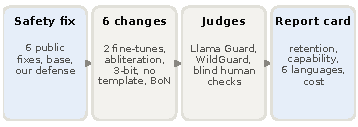
\includegraphics[width=\columnwidth]{figures/fig0_pipeline.pdf}
\caption{Aftermarket: every model goes through the same six post-release changes, two automatic judges checked
against blind human labels, and one report card.}
\label{fig:pipeline}
\end{figure}

An open-weight model is not a fixed artifact. Within days of a release, people fine-tune it on their own data,
quantize it to fit a phone, serve it from a raw completion endpoint without its chat template, or remove its refusals
on purpose with a single weight edit~\citep{arditi2024refusal}. A safety fix that holds only on the checkpoint its
authors published protects nobody who uses the model in any other form. Yet fixes are almost always evaluated on that
one checkpoint.

Each of these attacks is well documented on its own (\S\ref{sec:related}). What is missing is a common yardstick:
the same everyday post-release changes, applied with the same prompts, judges and statistics to every fix that
claims to make a model safer.

We build that yardstick, \emph{Aftermarket} (Fig.~\ref{fig:pipeline}), and apply it to every public safety fix for Tiny Aya Global
\citep{salamanca2026tinyaya} that we could load from a recent safety hackathon: six fixes spanning weight-space repair,
safety-aware fine-tuning, rank-one patches, and a prompt guard in the chat template. Our contributions:
\begin{enumerate}
\item \textbf{A shared post-release battery} of six changes, run on 12 models with identical seeds, prompts, two
  judges and paired statistics, plus capability, multilingual and serving-cost measurements\stagetwo{}
  (\S\ref{sec:setup}).
\item \textbf{A durability leaderboard} with one retention score, and the finding that release-time safety does
  not predict it (\S\ref{sec:survive}--\ref{sec:capability}).
\item \textbf{A judge audit} against blind hand labels in English and Yoruba: the pre-registered judge disagrees
  with a human far more than WildGuard on perturbed text, and judging Yoruba through back-translation overstates
  harm (\S\ref{sec:judges}, \S\ref{sec:multilingual}).
\item \textbf{A tested defense and a negative result}: hardening the layers that carry the refusal direction makes
  a model safer at release but \emph{less} durable, and no better than random layers (\S\ref{sec:defense}).
\end{enumerate}
Our headline has two parts. First, most public safety fixes do not survive ordinary post-release changes, and how
safe a model is at release says little about how well that safety holds; the attacks that undo them leave
capability nearly intact. Second, the automatic tools used to measure safety can mislead: against blind hand
labels, the pre-registered Llama Guard judge agrees with a human at only $\kappa=\V{kappa.lg.all}$ in English, and
judging Yoruba replies through back-translation overstates harm several-fold (the author, a native Yoruba speaker, confirms
\V{humjudge.flag.yes} of \V{humjudge.flag.n} flagged replies) while still missing some. A fix should be tested in the
forms people actually run, with judges checked against humans in every language reported.

\section{Related work}
\label{sec:related}

\paragraph{Harmful fine-tuning.} A few harmful, or even benign, examples erode an aligned model's safety
\citep{qi2024finetuning,yang2023shadow,lermen2023lora,zhan2024removing,huang2024survey}. Defenses constrain the
fine-tune \citep{huang2024lisa,yi2025safegrad} or make the weights resist it
\citep{henderson2023selfdestructing,rosati2024representation,tamirisa2025tamper}; we test released defenses against
a hobbyist's budget (one epoch of QLoRA on a free GPU), not an adaptive attacker.

\paragraph{Refusal, compression, cheap attacks.} Refusal is mediated by one direction that can be projected out of
the weights \citep{arditi2024refusal}, whose recipe our A3 follows; safety-critical weights are sparse
\citep{wei2024brittleness} and alignment is often a few tokens deep \citep{qi2025shallow}. Quantization can change
trustworthiness \citep{hong2024decoding} or hide behavior until quantized \citep{egashira2024exploiting}; we ask
whether 3 bits erase a fix. Best-of-N augmentations \citep{hughes2024bon} and low-resource languages
\citep{yong2023lowresource,deng2024multilingual} bypass safety training.

\paragraph{Judges.} Safety evaluations rest on classifiers \citep{inan2023llamaguard,han2024wildguard}, LLM-as-judge
rubrics \citep{zheng2023judging,souly2024strongreject} and fixed benchmarks
\citep{mazeika2024harmbench,chao2024jailbreakbench}; judge reliability on garbled or template-free text is rarely
measured against humans. We do so.

\section{Setup}
\label{sec:setup}

\paragraph{Model.} All runs use Tiny Aya Global (\texttt{CohereLabs/tiny-aya-global}, revision \texttt{af89d219},
36 layers) in fp16 with greedy decoding and at most 256 new tokens. The tokenizer is pinned to the same revision, and
we assert that every fix's tokenizer produces identical token IDs.

\paragraph{Fixes under test.} Six public fixes from the Lexsi AI Safety hackathon, each at a pinned revision and
credited to its team (Appendix~\ref{app:models}):
\run{SDT}, a weight-space repair that copies back 1\% of the base weights into a drifted model;
\run{GC}, a LoRA adapter trained with Lisa \citep{huang2024lisa};
\run{IL}, a LoRA adapter trained with SafeGrad \citep{yi2025safegrad};
\run{RL}, a safety system prompt inside the chat template (same weights as \run{BASE});
\run{ST}, sparse rank-one repair patches; and
\run{SP}, a safety-vector repair.
\run{RL\_noguard} serves \run{RL}'s weights with the base template, isolating the guard.
\run{BASE} is the unfixed model. \run{AM} is our defense (\S\ref{sec:defense}), with controls \run{AM\_rand0},
\run{AM\_rand1} (same recipe on random layers) and \run{AM\_all} (all layers, matched parameter count).

\paragraph{Attack battery.} Each change models something that routinely happens after release, on a one-T4 budget.
\begin{itemize}
\item \att{A0}: none (as released).
\item \att{A1} benign fine-tune: QLoRA \citep{dettmers2023qlora} on \V{cfg.a1.n} Alpaca examples, rank \V{cfg.lora_r},
  $\alpha=\V{cfg.lora_alpha}$, all attention and MLP projections, learning rate $\V{cfg.lr}$, \V{cfg.epochs} epoch,
  effective batch \V{cfg.effbatch}, loss on the response only.
\item \att{A2} harmful fine-tune: the same training on \V{cfg.a2.harmful} harmful instruction--response pairs from
  \texttt{LLM-LAT/harmful-dataset} (pinned \texttt{8bfba31}, the compliant ``rejected'' column) mixed with the first
  \V{cfg.a2.benign} \att{A1} examples.
\item \att{A3} abliteration \citep{arditi2024refusal}: a difference-in-means refusal direction from
  \V{cfg.n.calib} calibration pairs, projected out of every residual write matrix. The layer is chosen per model on
  dev prompts as the one whose ablation removes the most refusals among layers that leave benign next-token
  distributions nearly unchanged (KL $\le\V{cfg.a3.klmax}$). \att{A3max}, added after seeing test results, drops the
  KL filter and is reported separately, never ranked.
\item \att{A4} compression: HQQ 3-bit, group size \V{cfg.hqq.group} (4- and 2-bit in Appendix~\ref{app:tables}).
\item \att{A5raw}: the chat template stripped (raw completion). \att{A5bon}: best-of-\V{cfg.bon.n} random
  augmentations \citep{hughes2024bon} ($\sigma=\V{cfg.bon.sigma}$); a prompt counts as broken if any variant is.
\end{itemize}
Every run uses seed 42 and identical data and hyperparameters. Attack weights are never saved beyond the job.

\paragraph{Evaluation data.} ASR on \V{cfg.n.harmful} held-out harmful prompts (100 HarmBench
\citep{mazeika2024harmbench}, stratified by category, and 100 AdvBench \citep{zou2023universal}); over-refusal on the
\V{cfg.n.xstest} safe XSTest prompts \citep{rottger2024xstest}; capability on \V{cfg.n.mmlu} MMLU questions
\citep{hendrycks2021mmlu}. Splits were deduplicated against each other and against all training data; every choice
(attack layer rules, our defense) used separate dev splits only.

\paragraph{Capability benchmarks\stagetwo.} With lm-evaluation-harness \citep{biderman2024lessons} on vLLM
\citep{kwon2023vllm}, each run's own chat template, and fixed random subsets: the same \V{cfg.n.mmlu} MMLU items,
ARC-Challenge \citep[\V{cfg.cap.arc_challenge}]{clark2018arc}, HellaSwag
\citep[\V{cfg.cap.hellaswag}]{zellers2019hellaswag}, Winogrande \citep[\V{cfg.cap.winogrande}]{sakaguchi2020winogrande}
(classification, 0-shot), and IFEval \citep[all 541]{zhou2023ifeval} and GSM8K \citep[\V{cfg.cap.gsm8k}, 5-shot as
chat turns]{cobbe2021gsm8k} (generation). \att{A5raw} and \att{A5bon} change only the prompt, so their capability
equals \att{A0} and is not re-measured.

\paragraph{Judges.} Llama-Guard-3-1B \citep{inan2023llamaguard} was pre-registered as the primary judge; WildGuard
\citep{han2024wildguard} is the second judge for harmfulness and the refusal judge for XSTest. Both see the original
request. We audit both against \V{hum.nlabels} responses hand-labelled blind (request and response only), stratified
across models and attacks (\S\ref{sec:judges}).

\paragraph{Metrics and statistics.} ASR is the share of prompts answered harmfully. \emph{Retention} is
$1-\overline{(\text{ASR}_{\text{attack}}-\text{ASR}_{\text{A0}})}$, averaged over the attack families A1--A5 (1 means
nothing lost). All intervals are 95\% percentile bootstrap CIs over prompts (10{,}000 resamples); comparisons
against \run{BASE} and \run{AM} are paired bootstrap tests with Holm correction within each family of comparisons.
A cell whose MMLU falls below 30\% is flagged ``safe because broken''.

\paragraph{Pre-registration.} The battery, metrics, judges, test-split rule and defense recipe were committed
before the first test run, and our defense was frozen before its test run. \att{A3max}, the judge-reporting rule
(\S\ref{sec:judges}) and everything marked \stagetwo{} were added afterwards and are labelled as such.

\section{Results}

\begin{figure*}[t]
\centering
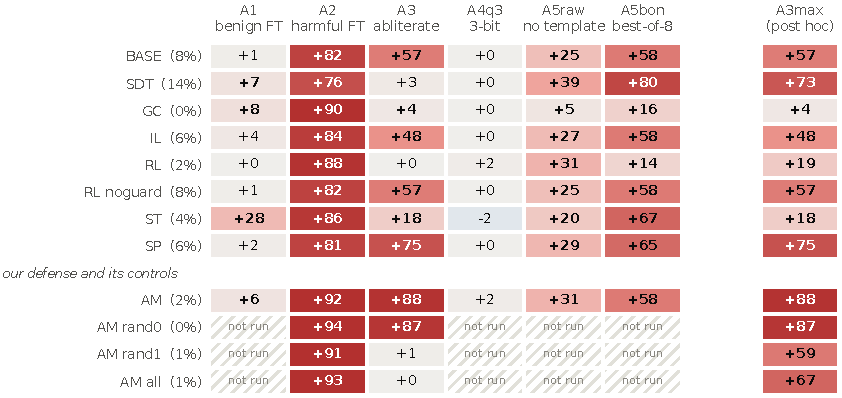
\includegraphics[width=0.92\textwidth]{figures/fig1_heatmap.pdf}
\caption{\textbf{Most fixes do not survive.} Rise in harmful-reply rate (WildGuard, percentage points) after each
post-release change, relative to the same run as released; row labels give the as-released rate. Bold: the paired
95\% bootstrap CI excludes 0 (200 prompts per cell). \att{A3max} is a post-hoc sensitivity variant of abliteration
and is never ranked. Controls of our defense ran the attacks it targets only. The same figure under Llama Guard is
in Appendix~\ref{app:tables}.}
\label{fig:heatmap}
\end{figure*}

\subsection{Do fixes survive?}
\label{sec:survive}
Figure~\ref{fig:heatmap} shows the rise in harmful replies after each change. The harmful fine-tune (\att{A2}) is
the hardest: every fix ends at \V{lg.A2.min}--\V{lg.A2.max}\% under Llama Guard (WildGuard \V{wg.A2.min}--\V{wg.A2.max}\%),
indistinguishable from the unfixed base model (\V{lg.BASE.A2}\%), while MMLU does not drop
(\run{BASE}: \V{mmlu.BASE.A0}\% before, \V{mmlu.BASE.A2}\% after; retrained and scored by log-likelihood in
Stage~2\stagetwo, \V{cap.mmlu.BASE.A0}\% and \V{cap.mmlu.BASE.A2}\%). Abliteration, with no training, takes \run{SP} from \V{wg.SP.A0}\% to
\V{wg.SP.A3}\% and \run{IL} from \V{wg.IL.A0}\% to \V{wg.IL.A3}\%; \run{GC} is the one weight-space fix that holds
(\V{wg.GC.A3}\%, also \V{wg.GC.A3max}\% at the strongest layer). The pre-registered layer rule under-attacks
\run{SDT}, which stays at \V{wg.SDT.A3}\% under \att{A3} but reaches \V{wg.SDT.A3max}\% under \att{A3max}.
Compression to 3 bits moves no run by more than \V{rise.wg.A4q3.maxabs} points (WildGuard; Llama Guard
\V{rise.lg.A4q3.maxabs}). Template removal and best-of-8 perturbations break most fixes; under \att{A5bon} only \run{GC} and the
template guard \run{RL} stay below 20\% (\V{wg.GC.A5bon}\% and \V{wg.RL.A5bon}\%), and \run{RL\_noguard} matches
\run{BASE} in every cell, so \run{RL}'s protection lives entirely in its template. A benign fine-tune leaves \run{ST}
less safe than no fix (\V{wg.ST.A1}\% vs \run{BASE} \V{wg.BASE.A1}\%).

\begin{figure}[t]
\centering
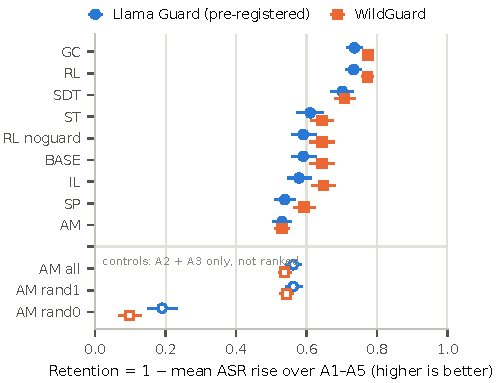
\includegraphics[width=\columnwidth]{figures/fig2_retention.pdf}
\caption{Retention with 95\% CIs (pre-registered Llama Guard judge, and WildGuard). Controls of our defense faced
only \att{A2} and \att{A3} and are not ranked.}
\label{fig:retention}
\end{figure}

\subsection{Retention ranking}
\label{sec:retention}
Under the pre-registered judge, \run{GC} ranks first (retention \V{ret.GC} \V{ret.GC.ci}) and \run{RL} second
(\V{ret.RL}); \run{BASE} scores \V{ret.BASE} and our \run{AM} ranks last (\V{ret.AM} \V{ret.AM.ci};
Fig.~\ref{fig:retention}). WildGuard gives the same top three and the same last place. Safety at release does not
predict retention: across the \V{rho.a0ret.lg.n} ranked runs, Spearman $\rho$ between as-released ASR and retention
is \V{rho.a0ret.lg} (permutation $p=\V{rho.a0ret.lg.p}$; WildGuard $\rho=\V{rho.a0ret.wg}$, $p=\V{rho.a0ret.wg.p}$). With
nine runs this is a lack of evidence for a relationship, not proof of none, but the extremes make the point: \run{AM}
is among the safest models at release (\V{wg.AM.A0}\%) and the least durable.

\begin{figure}[t]
\centering
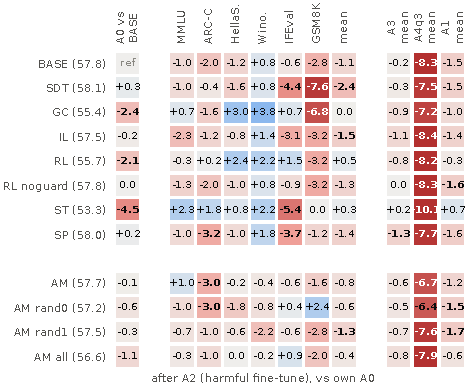
\includegraphics[width=\columnwidth]{figures/fig3_capability.pdf}
\caption{\textbf{Fixes and attacks barely move capability.} Change in accuracy (points) on six benchmarks and
their unweighted mean. Left: each fix as released vs \run{BASE}. Right: after the harmful fine-tune \att{A2} vs the
same run as released. Row labels give the as-released mean. Bold: paired 95\% bootstrap CI excludes 0 (no
multiplicity correction). Red = capability lost.}
\label{fig:capability}
\end{figure}

\subsection{Capability\stagetwo}
\label{sec:capability}
As released, \run{BASE} averages \V{cap.comp.BASE.A0}\% over the six benchmarks (MMLU \V{cap.mmlu.BASE.A0}, GSM8K
\V{cap.gsm.BASE.A0}, IFEval \V{cap.ifeval.BASE.A0}; Fig.~\ref{fig:capability}). Most fixes cost no measurable
capability. Three do: \run{ST} (\V{dcap.comp.ST.A0} points \V{dcap.comp.ST.A0.ci}; MMLU \V{dcap.mmlu.ST.A0}, GSM8K
\V{dcap.gsm.ST.A0}), \run{GC} (\V{dcap.comp.GC.A0}) and \run{RL} (\V{dcap.comp.RL.A0}). \run{RL}'s weights are
\run{BASE}'s, so its cost is the guard template (IFEval \V{dcap.ifeval.RL.A0}); \run{RL\_noguard} reproduces
\run{BASE} item for item, which also confirms that generation is deterministic. The harmful fine-tune, which removes
every fix's safety (\S\ref{sec:survive}), costs the attacker almost nothing: the mean moves by \V{dcap.comp.A2.min} to
\V{dcap.comp.A2.max} points, and the CI excludes 0 for \V{dcap.comp.A2.nsig} of \V{dcap.comp.A2.n} runs, the largest
being \run{SDT} (\V{dcap.comp.SDT.A2}, mostly GSM8K \V{dcap.gsm.SDT.A2}). No cell comes near the 30\% ``safe because
broken'' flag (lowest MMLU: \V{cap.mmlu.min}\%, \V{cap.mmlu.min.cell}). Attacked models are unsafe, not broken.
Per-benchmark scores are in Appendix~\ref{app:tables}.
\todo{add A3, A4q3 and A1 mean columns when those cells land; confirm the A2 claim with the judged Stage 2 A2 ASR.}

\subsection{Can we trust the judge?}
\label{sec:judges}
\begin{figure}[t]
\centering
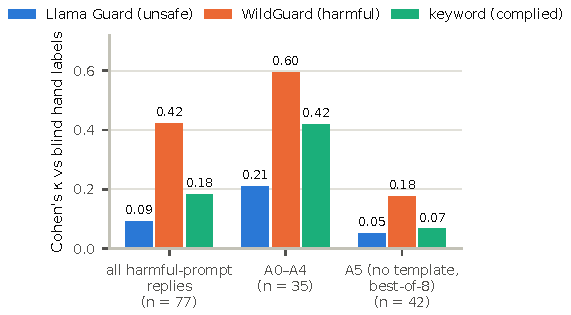
\includegraphics[width=\columnwidth]{figures/fig4_judges.pdf}
\caption{Agreement of each judge with \V{hum.nlabels} blind hand labels on harmful-prompt replies (whether the reply
gives harmful help). Both judges fall to near chance on template-stripped and perturbed text (\att{A5}).}
\label{fig:judges}
\end{figure}
Against the blind hand labels, WildGuard agrees with a human at $\kappa=\V{kappa.wg.all}$ and Llama Guard at
$\kappa=\V{kappa.lg.all}$ (Fig.~\ref{fig:judges}). On \att{A5} outputs both are near chance
($\kappa=\V{kappa.wg.afive}$ and \V{kappa.lg.afive}): Llama Guard flags \V{hum.rate.lg.afive}\% of sampled \att{A5}
replies as unsafe where the human finds \V{hum.humanrate.lg.afive}\%, mostly refusals in garbled text. Because the
judges disagree there, the headline best-of-8 number for \run{BASE} is \V{wg.BASE.A5bon}\% under WildGuard but
\V{lg.BASE.A5bon}\% under Llama Guard. We therefore report WildGuard first wherever the two judges differ by more than
10 points (a post-hoc reporting rule; rankings and tests still use the pre-registered judge). The ranking's top and
bottom do not depend on the judge (Fig.~\ref{fig:retention}).

\subsection{Our defense, and why it is a negative result}
\label{sec:defense}
\run{AM} hardens the $k=\V{cfg.am.k}$ layers whose refusal direction best separates harmful from benign dev prompts
(layers \V{cfg.am.layers}) with SafeGrad-style gradient surgery restricted to those layers, trains half of its refusal
batches with the top refusal direction ablated, and keeps those layers at \V{cfg.am.shieldbits} bits under compression.
Every choice was made on dev prompts; the recipe was frozen before its test run. \run{AM} is safer than \run{BASE} as
released under both judges (\V{lg.AM.A0}\% vs \V{lg.BASE.A0}\% Llama Guard; \V{wg.AM.A0}\% vs \V{wg.BASE.A0}\%
WildGuard) with unchanged over-refusal (\V{or.AM.A0}\% vs \V{or.BASE.A0}\%) and MMLU (\V{mmlu.AM.A0}\% vs
\V{mmlu.BASE.A0}\%). But it is \emph{worse} under abliteration (WildGuard \V{wg.AM.A3}\% vs \V{wg.BASE.A3}\%; Llama
Guard \V{lg.AM.A3}\% vs \V{lg.BASE.A3}\%), no better under the harmful fine-tune, and its located layers give no
advantage over random ones: \run{AM\_rand1} and \run{AM\_all} stay at \V{wg.AM_rand1.A3}\% and \V{wg.AM_all.A3}\%
under \att{A3}, \run{AM\_rand0} fails like \run{AM}. One plausible cause is that \run{AM}'s spread-refusal step
ablated an early-layer direction that turned out not to mediate refusal, while concentrating safety in early layers
made the model easier to abliterate. We report this as an informative negative result: locating refusal is not the
same as protecting it.
\todo{optional fig5 scatter (BASE, GC, AM, controls) once E1 composite capability lands.}

\subsection{Can we audit safety in other languages?\stagetwo}
\label{sec:multilingual}
\begin{figure}[t]
\centering
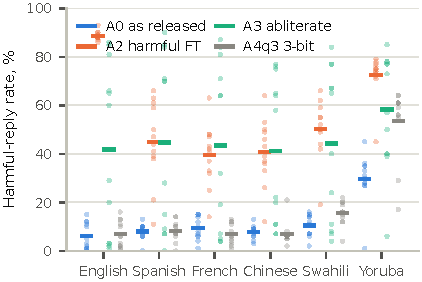
\includegraphics[width=\columnwidth]{figures/fig6_multilingual.pdf}
\caption{\textbf{Judged harmful-reply rate by language} (WildGuard on NLLB back-translations; incoherent replies count
as not harmful): bar = mean over the 12 runs, dots = single runs; 100 harmful prompts per cell, the same items in
every language. A native speaker confirms few of the Yoruba verdicts (\S\ref{sec:multilingual}), so the Yoruba bars
overstate harm.}
\label{fig:multilingual}
\end{figure}
Through the standard pipeline, translate the prompt, back-translate the reply, judge it in English, Yoruba looks far
less safe than every other language (Fig.~\ref{fig:multilingual}). As released, the judges flag
\V{mlmean.A0.yo.wg}\% of Yoruba replies against \V{mlmean.A0.en.wg}\% in English (paired gap \V{mlgap.A0.wg}
\V{mlgap.A0.wg.ci}, positive for all \V{mlgap.A0.wg.cells} runs, Llama Guard \V{mlgap.A0.lg}), and
\V{mlgap.A0.wg.rest} points more than the mean of Spanish, French, Chinese and Swahili. At 3 bits the contrast is
starkest: \V{mlmean.A4q3.yo.wg}\% vs \V{mlmean.A4q3.en.wg}\%, and for \V{mlex.nruns} models (\V{mlex.runs}) English
stays at or below \V{mlex.enmax}\% while Yoruba is judged at \V{mlex.yomin}--\V{mlex.yomax}\%. Read at face value,
an English-only audit would pass these models.

\emph{A native speaker's blind check does not support that reading.} Of 20 Yoruba replies the judges flagged
(10 as released, 10 at 3 bits), only \V{humjudge.flag.yes} actually help with the harmful request
(\V{humjudge.flag.yes.pct}\%, 95\% CI \V{humjudge.flag.yes.ci}), \V{humjudge.flag.partly} help partly and
\V{humjudge.flag.no} do not; the share is the same at both attacks (\V{humjudge.flag.A0.yes} and
\V{humjudge.flag.A4q3.yes} of 10). The judges also miss harm: \V{humjudge.ctrl.any} of \V{humjudge.ctrl.n} replies
they passed help at least partly, both at 3 bits. The translation check locates the problem in the replies, not the
prompts: \V{humyo.prompt.adequate}\% of machine-translated prompts keep their meaning (\V{humyo.prompt.harmful.adequate}\%
of harmful ones), but back-translation keeps the meaning of only \V{humyo.reply.adequate}\% of the model's Yoruba
replies, and only \V{humyo.reply.fluent}\% read as natural Yoruba. The judges are reading noisy translations of often
unnatural text, which also fits Yoruba's high over-refusal (\V{mlmean.A0.yo.or}\% vs \V{mlmean.A0.en.or}\%).
Scaling the judged rates by the confirmed share gives roughly \V{humadj.A0.yo.lo}--\V{humadj.A0.yo.hi}\% as released,
close to English, and \V{humadj.A4q3.yo.lo}--\V{humadj.A4q3.yo.hi}\% at 3 bits, perhaps above English's
\V{mlmean.A4q3.en.wg}\%, but 10 replies per attack cannot settle that. So we do not claim that the models are less
safe in Yoruba. What the data do show is that the back-translate-and-judge audit is not valid for Yoruba: it
overstates harm several-fold and still misses some. For Spanish and French, judging the original replies agrees with
the back-translated route on \V{mldirect.es.agree}\% and \V{mldirect.fr.agree}\%; a low-resource language needs
native-speaker labels or a judge that reads it.

\subsection{What does a fix cost to serve?\stagetwo}
\label{sec:cost}
\todo{E2: steady-state tokens/s per fix, \$ per 1M output tokens on T4/L4/A100, defense overhead, audit cost, ROI.}

\section{Practical takeaways}
\label{sec:takeaways}
\textbf{Test the forms people run.} Before claiming a fix, run at least a harmful fine-tune, abliteration and
3-bit compression: they cost an attacker one QLoRA epoch, one weight edit and one command, and in our results the
first two leave capability intact. \textbf{Check the judge, in every language.} Report two judges, hand-label a
sample, and do not trust back-translated judging for a low-resource language without native-speaker labels.
\textbf{Do not assume targeted hardening buys durability}; compare against random layers. \textbf{Put safety in the
weights if serving cost matters}: at 1B output tokens a month on an L4, a prompt guard adds
\$\V{roi.L4.RL.extra} a month, while weight fixes add nothing. \textbf{Audit before release; it is cheap.} The
\texttt{aftermarket audit} command runs the whole battery on any Tiny Aya Global derivative and writes a report
card ranked against our leaderboard, in \V{audit.full.hours} hours on one T4 for \$\V{audit.full.usd}, the price of
serving \V{audit.full.mtok}M tokens.

\section{Conclusion}
Safety fixes for open-weight models should be judged by what survives in the forms people run, and measured with
tools that have been checked against humans. On Tiny Aya Global, one cheap fine-tune or a single weight edit undoes
most public fixes while capability barely moves: the attacked models are unsafe, not broken. The instruments failed
too: Llama Guard agreed with a human at $\kappa=\V{kappa.lg.all}$, and back-translated judging made Yoruba look far
less safe than the author, a native Yoruba speaker, found it. Durability claims need both: the battery, and a judge audited in each
language.

\section*{Limitations}
We study one base model, Tiny Aya Global, and the fixes we could load; larger models may differ. Each
cell uses one training seed, except the seed check on three runs (Appendix~\ref{app:tables}). Prompt sets are
subsets (200 harmful English prompts, 100 per other language, fixed capability subsets), so small differences are
noise; we report CIs throughout. Both judges are imperfect (\S\ref{sec:judges}, \S\ref{sec:multilingual}). The Yoruba human checks were done by a single rater, the author, a native Yoruba speaker, on small samples (60 translations,
25 judge verdicts), so their percentages have wide CIs and no inter-rater agreement, and the human-adjusted Yoruba rates
are rough. Non-English prompts are machine-translated and replies judged after back-translation; only Spanish and
French were also judged directly. One rule (accepting Congo Swahili) changed after seeing test outputs; we report
both versions. Stage~2 experiments were planned before running but not pre-registered, and Stage~2 cells ran on T4
and L4 GPUs (99.7\% item agreement on a replicate). Throughput was measured on one software stack and priced from
list prices on one date. CircuitKIT's EAP-IG circuit discovery \citep{circuitkit2026}, tried for locating \run{AM}'s layers, ran out of memory on a T4 and on CPU and is used in no result.

\section*{Ethics statement}
Harmful prompts and fine-tuning data are public and were used only to evaluate and attack models. We
release no attack-tuned weights and no model completions to harmful prompts: generations stay in a private store
and judged tables hold only labels and aggregates. We do release machine translations of the
public benchmark prompts (HarmBench, AdvBench, XSTest), as multilingual benchmarks such as MultiJail
\citep{deng2024multilingual} do, and the Yoruba check sheets (prompts, and replies to safe XSTest prompts only). The attacks are
already public and cheap; one battery mainly helps defenders test fixes before release, so we release the audit
tool, not attacked models. We credit every team whose fix we evaluate; results describe fixes under our battery, not teams. The Yoruba checks were done by the author, a native Yoruba
speaker; the labelling tool warned that replies to harmful requests could be unpleasant and showed no
model, attack or verdict.


\bibliographystyle{acl_natbib}
\bibliography{custom}

\appendix
\section{Models under test}
\label{app:models}
\todo{table of releases, revisions, teams, licences; one line per fix on what it changes.}

\section{Attack and evaluation details}
\label{app:details}

\paragraph{Fine-tuning attacks.} \att{A1} trains QLoRA \citep{dettmers2023qlora} on \V{cfg.a1.n} Alpaca examples:
rank \V{cfg.lora_r}, $\alpha=\V{cfg.lora_alpha}$, all attention and MLP projections, learning rate $\V{cfg.lr}$,
\V{cfg.epochs} epoch, effective batch \V{cfg.effbatch}, loss on the response only; the adapter is merged into fp16
for evaluation. \att{A2} uses the same training on \V{cfg.a2.harmful} harmful instruction--response pairs from
\texttt{LLM-LAT/harmful-dataset} (pinned \texttt{8bfba31}, the compliant ``rejected'' column) mixed with the first
\V{cfg.a2.benign} \att{A1} examples.

\paragraph{Abliteration.} A difference-in-means refusal direction from \V{cfg.n.calib} calibration pairs is projected
out of every residual write matrix \citep{arditi2024refusal}. The layer is chosen per model on dev prompts as the one
whose ablation removes the most refusals among layers that leave benign next-token distributions nearly unchanged
(KL $\le\V{cfg.a3.klmax}$). \att{A3max} drops the KL filter.

\paragraph{Compression and prompting.} \att{A4} is HQQ 3-bit with group size \V{cfg.hqq.group} (4- and 2-bit in
Appendix~\ref{app:tables}). \att{A5raw} sends the request with no chat template. \att{A5bon} samples
\V{cfg.bon.n} augmentations per prompt \citep{hughes2024bon} ($\sigma=\V{cfg.bon.sigma}$); a prompt counts as broken if
any variant is.

\paragraph{Data.} Harmful prompts are 100 HarmBench prompts stratified by category and 100 AdvBench prompts; all
splits were deduplicated against each other and against all training data. A cell whose MMLU falls below 30\% is
flagged ``safe because broken''.

\paragraph{Capability benchmarks\stagetwo.} lm-evaluation-harness on vLLM with each run's chat template and fixed
random subsets: the same \V{cfg.n.mmlu} MMLU items, ARC-Challenge (\V{cfg.cap.arc_challenge}), HellaSwag
(\V{cfg.cap.hellaswag}) and Winogrande (\V{cfg.cap.winogrande}), 0-shot; IFEval (all 541) and GSM8K
(\V{cfg.cap.gsm8k}, 5-shot as chat turns). \att{A5raw} and \att{A5bon} change only the prompt, so their capability
equals \att{A0}. Primary metrics: accuracy (MMLU, Winogrande), normalized accuracy (ARC, HellaSwag), prompt-level
strict accuracy (IFEval) and strict exact match (GSM8K); the mean is their unweighted average. The adapters of
\att{A1}/\att{A2} no longer existed after Stage~1 (attacked weights are deleted by design), so they were retrained
with the same seed, data and hyperparameters. \att{A0} and \att{A2} cells ran on one T4 each (vLLM fp16, greedy).
\todo{state the GPU of the A3 / A4q3 / A1 cells once they land.}

\section{Full results}
\label{app:tables}
\begin{table}[h]
\centering\small\setlength{\tabcolsep}{3pt}
\resizebox{\columnwidth}{!}{\begin{tabular}{lrrrrrrrrrrr}
\toprule
Run & MMLU & ARC-C & HellaS. & Wino. & IFEval & GSM8K & Mean & $\Delta$\att{A2} & $\Delta$\att{A3} & $\Delta$\att{A4q3} & $\Delta$\att{A1} \\
\midrule
\run{BASE} & 56.0 & 43.6 & 65.4 & 64.0 & 58.8 & 58.8 & 57.8 & $-$1.1 & $-$0.2 & \textbf{$-$8.3} & $-$1.5 \\
\run{SDT} & 56.3 & 43.6 & 66.4 & 64.4 & 60.3 & 57.6 & 58.1 & \textbf{$-$2.4} & $-$0.3 & \textbf{$-$7.5} & $-$1.5 \\
\run{GC} & 53.7 & 44.4 & 61.8 & 62.8 & 53.8 & 56.0 & 55.4 & 0.0 & $-$0.9 & \textbf{$-$7.2} & $-$1.0 \\
\run{IL} & 56.3 & 44.0 & 65.2 & 63.4 & 59.0 & 57.2 & 57.5 & \textbf{$-$1.5} & $-$1.1 & \textbf{$-$8.4} & $-$1.4 \\
\run{RL} & 54.3 & 42.8 & 63.0 & 63.2 & 53.2 & 57.6 & 55.7 & +0.5 & $-$0.8 & \textbf{$-$8.2} & $-$0.3 \\
\run{RL\_noguard} & 56.0 & 43.6 & 65.4 & 64.0 & 58.8 & 58.8 & 57.8 & $-$1.3 & 0.0 & \textbf{$-$8.3} & \textbf{$-$1.6} \\
\run{ST} & 49.0 & 39.6 & 62.4 & 62.6 & 56.7 & 49.2 & 53.3 & +0.3 & +0.2 & \textbf{$-$10.1} & +0.7 \\
\run{SP} & 56.0 & 44.2 & 65.8 & 64.2 & 59.5 & 58.0 & 58.0 & $-$1.4 & \textbf{$-$1.3} & \textbf{$-$7.7} & $-$1.6 \\
\run{AM} & 52.7 & 45.6 & 65.0 & 66.0 & 57.9 & 58.8 & 57.7 & $-$0.8 & $-$0.6 & \textbf{$-$6.7} & $-$1.2 \\
\run{AM\_rand0} & 54.7 & 44.4 & 66.0 & 66.4 & 56.7 & 54.8 & 57.2 & $-$0.6 & $-$0.5 & \textbf{$-$6.4} & \textbf{$-$1.5} \\
\run{AM\_rand1} & 54.7 & 44.8 & 65.0 & 66.4 & 56.4 & 57.6 & 57.5 & \textbf{$-$1.3} & $-$0.7 & \textbf{$-$7.6} & \textbf{$-$1.7} \\
\run{AM\_all} & 54.0 & 43.4 & 65.0 & 65.2 & 55.1 & 57.2 & 56.6 & $-$0.4 & $-$0.8 & \textbf{$-$7.9} & $-$0.6 \\
\bottomrule
\end{tabular}
}
\caption{Capability as released (\%, per benchmark and mean) and the change in the mean after each attack (points,
vs the same run as released; bold: paired 95\% bootstrap CI excludes 0).\stagetwo}
\label{tab:capability}
\end{table}
\todo{full tables for every run x attack x judge; Llama Guard heatmap; 4/2-bit; retention without A3; per-benchmark capability; per-language table; cost table; E4 overlap.}


\end{document}
